\documentclass[PhD]{uclathes}

% Packages
%\usepackage[T1]{fontenc} % Allows for 8-bit font encoding
\usepackage{setspace} % Sets space between lines
\usepackage{animate,pdfpages} % Allow for animated figures, importing PDF figures, and converting EPS to PDF
\usepackage[space]{grffile} % Extended file name support for graphics
\usepackage{float} % Improved interface for floating objects
\usepackage{subcaption} % Allows for subfigures within figures
\usepackage{caption} % Captions in floating environments
\usepackage{array} % Extending the array and tabular environments
\usepackage{multirow} % Create tabular cells spanning multiple rows
\usepackage{gensymb} % Generic symbols for both text and math mode
\usepackage{amsmath,amssymb,amsfonts,amsthm,mathrsfs,mathtools,accents} % Various packages for math typesetting
\usepackage{adjustbox,relsize} % Set font size relative to the current font size
\usepackage[notrig]{physics} % Physics symbols and units
\usepackage{siunitx} % Physics units
\usepackage{cancel,slashed} % Place lines through math and slashes through characters
\usepackage{xparse} % Generic document command parser
\usepackage{tikz,tikz-3dplot,circuitikz,pgfplots,tikz-cd,tikz-feynman} % Drawing environments
\usepackage{centernot} % Centered \not command
\usepackage{xcolor} % Color extensions for LaTeX and pdfLaTeX
\usepackage{listings} % Typeset text in WYSIWYG style and source code listings
\usepackage{fancyvrb} % Sophisticated verbatim text
\usepackage{lastpage} % Reference last page for Page N of M type footers
\usepackage[percent]{overpic} % Combine LaTeX commands over included graphics
\usepackage{empheq} % Emphasizing equations
\usepackage{comment} % Allows for commenting out large blocks of code
\usepackage[title]{appendix} % Customization of appendices
\usepackage{simpler-wick} % Allows for Wick contractions
\usepackage[htt]{hyphenat} % Enables hyphenation in \texttt environments
\usepackage{url} % Allows for \path command for long file paths
\usepackage[hidelinks,colorlinks=false]{hyperref} % Allow for hyperlinks
\usepackage{bookmark} % Automatically create bookmarks
\usepackage{xspace} % Allows for \xspace command to check if a space is needed
\usepackage{cite} % Makes citations with multiple references look better


% Configure TikZ
\input{preamble/tikz.tex}

% Configure listings
\input{preamble/listings.tex}

% Configure captions
\captionsetup[table]{font={stretch=1.5}}
\captionsetup[figure]{font={stretch=1.5}}

% Configure itemize layers
\renewcommand{\labelitemii}{\ensuremath{\circ}}

% Enable bold math in section titles
\makeatletter
\g@addto@macro\bfseries{\boldmath}
\makeatother

% Commands
\renewcommand\qedsymbol{$\blacksquare$} % Change QED symbol to solid black box
\newcommand\numberthis{\addtocounter{equation}{1}\tag{\theequation}} % Number equations in align* environments

\sisetup{inter-unit-product=\ensuremath{{}\cdot{}}} % Change symbol for products of physical units
\renewcommand{\unit}{\ \si} % Define physical unit command with proper spacing
\DeclareSIUnit\clight{\text{\ensuremath{c}}} % Redefine speed of light so that it has no subscript

% Redefine command for unit vectors to add space
\let\oldvu\vu
\makeatletter
\renewcommand{\vu}{\@ifstar{\mathop{}\!\oldvu*}\mathop{}\!\oldvu}
\makeatother

% Create spacing for equals sign in align environments
\newcommand{\equad}{\mathrel{\phantom{=}}}

% Alphabet for blackboard bold numbers
\newcommand{\bbfamily}{\fontencoding{U}\fontfamily{bbold}\selectfont}
\DeclareMathAlphabet{\mathbbold}{U}{bbold}{m}{n}

\newcommand{\lumi}{\mathcal{L}} % Luminosity
\newcommand{\intlumi}{\mathcal{L}_\mathrm{int}} % Integrated luminosity
\newcommand{\pt}{\ensuremath{p_\mathrm{T}}\xspace} % Transverse momentum


\title{
	Search for Long-Lived Particles Decaying to Photon Pairs in Rare Higgs Boson Decays using 13 TeV Proton-Proton Collisions at the Compact Muon Solenoid
}

\author{Tyler Christopher Lam}
\department{Physics}
\degreeyear{2024}

\chair{Michalis Bachtis}
\member{Davlid Saltzberg}
\member{Jay Hauser}
\member{Thomas Dumitrescu}
\dedication{
	\textit{
		To my parents, Jean and Bobby, for their love and support from across the country
	}
}

\acknowledgments{
First and foremost, no one has contributed more to my success as a graduate student than my advisor, Michalis Bachtis. The first summer I spent researching for him cemented my desire to study experimental particle physics. From there, his dedication, enthusiasm, and mentorship were indispensable during my journey through graduate school.  I do not know of any advisor who is more available to their students and is more willing to perform hands-on work to help in a project. Thank you for everything, Michalis.

More thanks goes to the current and former members of the UCLA CMS research group. Thank you to my former officemates David Hamilton and Maxx Tepper; our workplace shenanigans gave me something to look forward to during slow days at work. I would also like to thank the other CMS graduate students from when I arrived at UCLA: Brent Stone, Will Nash, and Chris Schnaible for welcoming me into the group and our countless thought-provoking lunch discussions. Lastly, a thanks to the remaining graduate students, engineers, and postdocs Gael Flores-Avila, Antonett Prado, Abhishek Datta, Elisabetta Manca, Joseph Carlson, David Gotler, Alex Tan, and Delano Campos for making the office an enjoyable place to work.

My time at UCLA has been marked by countless friendships with students outside of the CMS research group as well. No words can express how important my former roommates Adam Trapp and Kyle Ferguson were towards maintaining my sanity during a global pandemic. Despite everything, I look back on our many (mis)adventures and remember this time fondly. You have been such an integral part of my time at UCLA that, to avoid repetition, I ask that put yourselves in any of the following thanks that apply to you. In a similar vein, thank you to Ronald Lopez and Rick Mebane for the weekly tennis sessions, which gave me an excuse to go outside during the lockdown. I would also like to thank Eric Cropp, Eddie Chang, Lukas Lindwasser, and Pratik Sathe for turning our comprehensive exam study group into a food-centric outing group.  To my friends that I have bonded with on the bouldering wall, I would like to thank Tony Pahl, Abhijah Simon, Akash Gupta, Rory Bentley, Will Flanagan, and Wes Armstrong. Finally, for making after-work and weekend board game nights fun I would like to thank Sarah Chase, Henry Wong, and Phil Travis.

Beyond UCLA, I would like to thank my parents, Bobby and Jean, who eventually learned not to ask a graduate student when they will graduate. My career as a physicist would never have been possible without them. Thank you to my sibling Ira for being a consistent moral and political compass. Additional thanks to Tor Raubenheimer -- my uncle, Stanford professor, and physicist at SLAC -- who inspired me to study physics in middle school when he joined our family. Last, but by no stretch of the imagination least, thank you to Levina Lin for being an unending source of stability and support over the last few years.

This thesis includes material that is based upon work supported by the U.S. Department of Energy under award number DE-SC0009937.
}

\vitaitem{2017}
{
	B.S\ (Physics) and B.A.\ (Mathematics),
	University of Virginia
}

\vitaitem{2017-2018}
{
	Teaching Assistant,
	Department of Physics and Astronomy,
	UCLA,
	Los Angeles, California
}

\vitaitem{2018}
{
	M.S.\ (Physics)
	UCLA
}

\vitaitem{2018-2024}
{
	Graduate Research Assistant,
	Department of Physics and Astronomy,
	UCLA
}

\abstract{
This thesis describes the search for rare Standard Model (SM) Higgs boson decays to long-lived scalar bosons ($\Phi$) decaying to photon pairs using data collected by the Compact Muon Solenoid (CMS) detector at the Large Hadron Collider. The data were collected from 2016, 2017, and 2018 proton-proton collisions at center-of-mass energy of $\sqrt{s}=13\TeV$ and correspond to an integrated luminosity of $138\unit{fb^{-1}}$. Events are triggered using the leptonic decays of the \PZ boson produced in association with the SM Higgs boson. Although the CMS electromagnetic calorimeter has limited vertex reconstruction capabilities for photons, this analysis utilizes a novel reconstruction technique using kinematic constraints to calculate the displaced vertices of the diphotons. Signal is extracted using a counting-based maximum-likelihood approach in bins of the diphoton vertex \lxy and the invariant photon mass. Results are interpreted in terms of upper limits on branching ratios $\mathcal{BR}(\PH\to\Phi\Phi)\times\mathcal{BR}(\Phi\to\PGg\PGg)$ and in terms of the model independent production cross section $\sigma(\PZ+\Phi\Phi)\times\mathcal{BR}(\Phi\to\PGg\PGg)$. No significant excess above SM expectation is observed.
}

\begin{document}

\makeintropages

% !TEX = root../thesis.tex

\chapter{Introduction}
\label{chap:intro}
Understanding the composition of matter and the forces that govern it are the core principles motivating particle physics. The idea that all matter is composed of some fundamental building block dates back to 440 B.C. in ancient Greece, where these blocks were referred to as \textit{atomos}, meaning ``indivisible''~\cite{wolfgang2019}. This is the origin of the modern \textit{atom}, coined in 1803 by John Dalton. In his atomic theory, Dalton proposed that all matter was composed of tiny, individual particles called atoms which could neither be created nor destroyed~\cite{oed_physics}. This theory held until 1897, when J.J. Thomson discovered that cathode rays emitted from a hot filament were actually beams of charged particles~\cite{thomson_electron}. Thomson theorized that atoms were not fundamental but composite particles, consisting of a positively charged ``paste'' with his charged particles, later named electrons, embedded within. Thomson's model of the atom was further refined in 1911, when Ernest Rutherford's gold foil experiment revealed that atoms consisted of a dense, charged core and resulted in the discovery of the proton~\cite{rutherford}. Finally, in 1932, the classical model of the atom was completed when James Chadwick discovered the neutron by observing radiation emitted from a beryllium target that was bombarded with alpha particles~\cite{chadwick}.

In parallel to classical atomic theory, quantum theory began to develop in 1900 when Max Planck solved the ultraviolet catastrophe -- a problem in which the power radiated from an ideal blackbody was calculated to be infinite -- by assuming that energy from electromagnetic radiation was quantized~\cite{kittel1980thermal}. This energy was revealed to be discrete particles with quantized energies following the work of Albert Einstein, through his explanation of the photoelectric effect in 1905, and A. H. Compton in 1923, through his discovery of Compton scattering. These particles, later named \textit{photons}, were the first interpretation of particles acting as mediators of a force.

The next question for particle physics was to determine the mechanism that held the nucleus together. Physicists were certain it must be a new force, as the protons would repel each other through the electromagnetic force and were much too light for gravity to play any significant role. In 1934, Yukawa proposed the first theory of the strong force and predicted a mediator particle with mass about one-sixth of the proton mass~\cite{QFTNutshell}. He called this intermediate particle a \textit{meson} -- a middle ground in mass between the light, electron scale particles (\textit{leptons}) and heavy, proton scale particles (\textit{baryons}). The search for this strong mediator eventually led to the discovery of both the pion (\PGp) and muon (\PGm)~\cite{pion_discovery}, with the pion being the meson Yukawa predicted and the muon being a lepton from the pion decay -- though neither were the true mediator of the strong force.

Throughout the next decade a myriad of new particles were discovered that verified theoretical predictions, such as the positron (and more generally antiparticles) in 1932 by C. D. Anderson~\cite{positron_discovery} and the neutrino in the 1950s by Cowan and Reines\cite{neutrino_discovery}. Additionally, several ``strange'' mesons and baryons were discovered using cloud chambers and particle accelerators, such as the kaon (\PKz) in 1947 by Rochester and Butler~\cite{kaon_discovery} and the lambda (\PGL) in 1950 by Hopper and Biswas~\cite{lambda_discovery}. In order to develop a unified model to accommodate all of the newly discovered particles, Gell-Mann and Nishijima independently devised the property of particle \textit{strangeness}~\cite{strangeness_gellmann,strangeness_nishijima}, eventually leading to Gell-Mann creating the Eightfold Way in 1961, which mapped baryons and mesons on an elegant, if not convoluted, grid of strangeness and electric charge~\cite{eightfoldway}. This grid had one notable gap, which Gell-Mann predicted would be a new particle and resulted in the discovery of the omega-minus (\PGOm) in 1964~\cite{omega_discovery}.

In 1964 Gell-Mann and Zweig independently proposed that baryons and mesons were not actually fundamental particles, but were instead composed of elementary particles called \textit{quarks}~\cite{gellmann_quarks,zweig_quarks}. Once again what scientists believed were the smallest constituents of matter were broken down into even smaller units. In this theory there are three quarks (\PQu, \PQd, and \PQs) that each carry a charge and strangeness, every meson is composed of a quark-antiquark pair, and every (anti)baryon is composed of three (anti)quarks. From this, the complex grid in Gell-Mann's Eightfold Way followed naturally by mapping every allowed combination of quarks. The first evidence supporting the quark theory came in 1969 from the Stanford Linear Accelerator Center (SLAC), in an experiment analogous to Rutherford's gold foil experiment, by scattering electrons off of protons and measuring the deflection~\cite{slac_quark}. Further evidence came in the form of the \PJGy meson discovery in November, 1974 from Brookhaven~\cite{jpsi_brookhaven} and SLAC~\cite{jpsi_slac}, which indicated the existence of a fourth flavor of quark -- the charm (\PQc).

The discovery of the \PJGy meson spurred what is known as the November revolution, a period of rapid discovery in the world of particle physics~\cite{revolution}. As expected, several baryons and mesons containing the charm quark were discovered, but the periodic table of fundamental particles gained several new entries as well. In 1975, the tau lepton (\PGt) was discovered along with its corresponding neutrino~\cite{tau_discovery}, and in 1977 the discovery of the upsilon meson (\PGU) indicated the existence of a fifth flavor of quark, the bottom (\PQb)~\cite{upsilon_discovery}. At this point, there were six leptons and five quarks, with the existence of a sixth quark predicted to maintain parity between the quarks and leptons. The final quark, dubbed the top (\PQt), was eventually discovered in 1995 at the Tevatron~\cite{top_discovery}, and is the last quark discovered as of present day.

The theory that describes the fundamental particles and the interaction forces is known as the Standard Model (SM). It perfectly describes the behavior of the quarks and leptons, though this is by construction as most of the parameters were determined empirically through experiment. For this reason, the predictive power of the SM was not truly validated until the discovery of the \PW, \PZ, and (most importantly) Higgs bosons. The first two are the force mediators of the weak force, which governs nuclear decay, and were predicted by Glashow, Weinberg, and Salem from their work on electroweak unification~\cite{ew_nobelprize} before being discovered in 1983 at the European Organization for Nuclear Research (CERN)~\cite{w_discovery,z_discovery}. The Higgs boson, which was predicted to give mass to the fundamental particles, managed to evade detection until the Large Hadron Collider began taking data in 2010. After two years of data taking the Higgs boson was finally discovered in 2012~\cite{higgs_atlas,higgs_cms}, marking a major milestone for the predictive power of the SM.

The discovery of the Higgs boson was the last missing piece of the Standard Model, but the puzzle of fundamental particles is still incomplete. Dark matter, which comprises 27\% of mass-energy of the observable universe, is not predicted by any SM particle. Moreover, there is no evidence for the existence of stable antimatter in the universe and no mechanism in the Standard Model that fully explains this matter-antimatter asymmetry. If gravity is to be incorporated into the SM, then it must be quantized, similar to Einstein and his quantization of light, but gravity and general relativity are thought to be incompatible with quantum theory~\cite{sm_grav}. Neutrinos, which are assumed by the SM to be massless, have experimentally been shown to have non-zero mass. Theories seeking to resolve these issues are referred to as Beyond the Standard Model (BSM), and are the motivation for several ongoing experiments at the LHC.

This thesis describes a search for Higgs boson decays to long-lived, BSM bosons ($\Phi$) known as  which then decay to two photons. These long-lived particles (LLPs) are predicted in several BSM theories, hence the analysis is intended to be independent of the specific theoretical model to provide maximum discovery potential. The data used in this analysis correspond to proton-proton collisions with center-of-mass energy of 13\TeV collected by the Compact Muon Solenoid (CMS) detector at the LHC from 2016-2018. In order to provide the full context for the analysis, chapter~\ref{chap:theory} will give a brief overview of the Standard Model and the theoretical motivation for LLPs. Greater detail on the mathematical formalism of the Standard Model and quantum field theory can be found in appendix~\ref{sec:sm_theory}. Chapter~\ref{chap:exp} then describes the LHC and CMS detector used to obtain the data for this analysis, with chapter~\ref{chap:kbmtf} detailing work done for the real time muon reconstruction done by the level-1 trigger in CMS. The full $\PH\to\Phi\Phi\to\PGg\PGg+X$ analysis itself is then given in chapter~\ref{chap:ana}.
% !TEX = root../thesis.tex

\chapter{The Standard Model and Motivations for Displaced Photons}
\label{chap:theory}
In this chapter, we present an overview of the Standard Model (SM) -- the best current description of the fundamental constituents of matter and the interactions between them. We begin with a brief description of the SM particles, followed by an outline of the mechanism that determines particle lifetimes. This establishes the groundwork to discuss the Higgs boson its relation to long-lived, beyond the standard model particles that motivate the $\PH\to\Phi\Phi\to\PGg\PGg+X$ analysis presented in chapter~\ref{chap:ana}.

\section{Elementary Particles in the Standard Model} \label{sec:SM}
The Standard Model is a quantum field theory that describes interactions between fundamental particles (see appendix~\ref{sec:sm_theory_qft} for a description of the mathematical formalism). According to the SM, all matter is composed of spin-1/2 particles known as fermions with forces that interact via fields mediated by spin-1 gauge bosons. Of the four forces -- gravity, electromagnetic, weak, and strong -- the SM provides a description of all but gravity (see appendix~\ref{sec:sm_theory_gauge}). The spin-1/2 fermions can be divided into three generations of increasing mass, with each generation divided into a quark doublet and lepton doublet. The gauge bosons are composed of the photon ($\PGg$) which mediates the electromagnetic force, the \PZ and \PWpm bosons which mediate the weak force, and 8 gluons (\Pg) which mediate the strong force. The \PZ and \PW bosons gain mass through a process known as the Higgs mechanism, which predicts the existence of a scalar boson \PH known as the Higgs boson. This process is presented in detail in section~\ref{sec:sm_theory_higgs}. Figure~\ref{tab:SM} shows the mass, charge, and spin of the fermions grouped by generation, the gauge bosons, and the Higgs boson. Each fermion has an associated antiparticle with identical spin and mass but opposite electrical charge.

\begin{figure}[htb!]
	\centering
	% !TEX = root../../thesis.tex

% Colors from https://latexcolor.com/
\definecolor{aqua}{rgb}{0.5, 1.0, 1.0}
\definecolor{spring}{rgb}{0..65, .99, 0.0}
\definecolor{brick}{rgb}{.8, .25, .33}
\definecolor{ube}{rgb}{0.82, 0.62, 0.91}

\begin{tikzpicture}
	\coordinate (u) at (0,0);
	\coordinate (d) at (0, -2.15);
	\coordinate (c) at (2.15, 0);
	\coordinate (s) at (2.15, -2.15);
	\coordinate (t) at (4.3, 0);
	\coordinate (b) at (4.3, -2.15);
	\coordinate (e) at (0, -4.3);
	\coordinate (mu) at (2.15, -4.3);
	\coordinate (tau) at (4.3, -4.3);
	\coordinate (ne) at (0, -6.45);
	\coordinate (nmu) at (2.15, -6.45);
	\coordinate (ntau) at (4.3, -6.45);
	\coordinate (glu) at (6.75, 0);
	\coordinate (g) at (6.75, -2.15);
	\coordinate (z) at (6.75, -4.3);
	\coordinate (w) at (6.75, -6.45);
	\coordinate (h) at (9.20, 0);
	
	% quarks
	\draw pic at (u) {particle={aqua!50}{$\PQu$}{up}{$2.16\MeVcc$}{$2/3$}{$1/2$}}; %Up quark
	\draw pic at (d) {particle={aqua!50}{$\PQd$}{down}{$4.70\MeVcc$}{$-1/3$}{$1/2$}}; % Down quark
	\draw pic at (c) {particle={aqua!50}{$\PQc$}{charm}{$1.27\GeVcc$}{$2/3$}{$1/2$}}; %Charm
	\draw pic at (s) {particle={aqua!50}{$\PQs$}{strange}{$93.5\MeVcc$}{$-1/3$}{$1/2$}}; %Strange
	\draw pic at (t) {particle={aqua!50}{$\PQt$}{top}{$172.57\GeVcc$}{$2/3$}{$1/2$}}; %Top
	\draw pic at (b) {particle={aqua!50}{$\PQb$}{bottom}{$4.183\GeVcc$}{$-1/3$}{$1/2$}}; %Bot
	
	% leptons
	\draw pic at (e) {particle={spring!35}{$\Pe$}{electron}{$511\keVcc$}{$-1$}{$1/2$}};
	\draw pic at (mu) {particle={spring!35}{$\PGm$}{muon}{$105.66\MeVcc$}{$-1$}{$1/2$}}; 
	\draw pic at (tau) {particle={spring!35}{$\PGt$}{tau}{$1.776\GeVcc$}{$-1$}{$1/2$}}; 
	\draw pic at (ne) {particle={spring!35}{$\PGne$}{\Pe neutrino}{$<1.1\eVcc$}{$0$}{$1/2$}};
	\draw pic at (nmu) {particle={spring!35}{$\PGnGm$}{\PGm neutrino}{$<0.17\MeVcc$}{$0$}{$1/2$}};
	\draw pic at (ntau) {particle={spring!35}{$\PGnGt$}{\PGt neutrino}{$<18\MeVcc$}{$0$}{$1/2$}};	
	
	% gauge bosons
	\draw pic at (glu) {particle={brick!30}{$\Pg$}{gluon}{$0$}{$0$}{$1$}};
	\draw pic at (g) {particle={brick!30}{$\PGg$}{photon}{$0$}{$0$}{$1$}};
	\draw pic at (z) {particle={brick!30}{$\PZ$}{Z boson}{$91.188\GeVcc$}{$0$}{$1$}};
	\draw pic at (w) {particle={brick!30}{$\PW$}{W boson}{$80.37\GeVcc$}{$\pm1$}{$1$}};
	
	% Higgs
	\draw pic at (h) {particle={ube!50}{$\PH$}{Higgs boson}{$125.2\GeVcc$}{0}{0}};
	
	% Labels
	\node at ($(u)+(-1, 0.8)$) [anchor=mid east, scale=0.6] {mass};
	\node at ($(u)+(-1, 0.5)$) [anchor=mid east, scale=0.6] {charge};
	\node at ($(u)+(-1, 0.2)$) [anchor=mid east, scale=0.6] {spin};
	
	\node at ($(u)+(0, 1.35)$) {I};
	\node at ($(c)+(0, 1.35)$) {II};
	\node at ($(t)+(0, 1.35)$) {III};	
	%\node at ($(c)+(0, 1.9)$) {Generations};
	\node at ($(u)+(-1,1.35)$) [anchor=east, scale=0.75] {Generation};
	
	\node at ($(d)+(-1.35, -1)$) [rotate=90,anchor=mid west, text=aqua!60!black] {Quarks};
	\node at ($(ne)+(-1.35, -1)$) [rotate=90,anchor=mid west, text=spring!60!black] {Leptons};
	\node at ($(w)+(1.35, -1)$) [rotate=90,anchor=mid west, text=brick!60!black] {Gauge Bosons};
\end{tikzpicture}

	\caption[Table of all Standard Model particles, divided by generation and particle type. Each particle is labeled with its mass, charge, spin, and symbol. Quarks are shown in blue, leptons in green, gauge bosons in red, and the Higgs boson in purple.]{Table of all Standard Model particles, divided by generation and particle type. Each particle is labeled with its mass, charge, spin, and symbol. Quarks are shown in blue, leptons in green, gauge bosons in red, and the Higgs boson in purple. Values taken from~\cite{Workman:2022ynf}.}
	\label{tab:SM}
\end{figure}

\subsection{Fermions} \label{sec:sm_quarks}
Quarks are fermions that interact with the strong, weak, and electromagnetic force. They are found exclusively in bound states known as hadrons. The two main types of hadrons are quark-antiquark pairs called mesons or three quark (or three antiquark) configurations known as baryons. For example, protons, the most commonly known baryons, are composed of two up quarks and one down quark (\PQuns\PQuns\PQdns), and the \PGpp is a meson composed of an up quark and a down antiquark (\PQuns\PAQdns). Each column of quarks in table~\ref{tab:SM} forms a doublet, with the upper quark having charge $+2/3$ while the lower quark has charge $-1/3$. Thus mesons can have charge 0 or $\pm$1 and baryons can have charge 0, $\pm$1, or $\pm$2.

Due to their interaction with the strong force, quarks carry one of three ``color'' charges of either red, blue, or green (or antired, antiblue, or antigreen). Although it is not theoretically required, it has been experimentally shown that quarks must always exist in a colorless bound state. Baryons must have one quark of each color (or anti-color), and mesons must consist of color-anticolor pairs. This property is known as color confinement.

Leptons are fermions consisting of three charged particles -- the electron, muon, and tau (\Pe, \PGm, and \PGt) -- and three corresponding neutral particles (\PGne, \PGnGm, and \PGnGt) called neutrinos. The charged leptons interact through both the electromagnetic and weak force, while the neutrinos interact only through the weak force. The lepton and neutrino doublets are intrinsically linked through the weak force. Neutrinos have extremely small masses compared to the other massive SM particles, and can undergo oscillations between flavors.

\subsection{Bosons} \label{sec:sm_bosons}
The gauge bosons are the spin-1 mediators of the electromagnetic, weak, and strong forces. The photon is the massless mediator of the electromagnetic force and couples to charged particles. Since they do not carry electric charge, photons do not directly interact with other photons. On the other hand, gluons, which are the massless mediators for the strong force, carry two color charges and can therefore interact with other gluons. Lastly, the \PZ and \PWpm bosons are the mediators of the weak force and can interact with all fermions as well as each other.

The Higgs boson is the only currently known scalar boson. In the SM, the \PZ and \PWpm bosons as well as all fermions are required to be massless due to various symmetry requirements. The Higgs mechanism, through a process known as spontaneous symmetry breaking, allows these particles to acquire non-zero mass without violating conservation laws. In this sense, the Higgs boson is said to give masses to the particles. The Higgs boson couples to any particle with mass, which includes itself, the aforementioned \PZ and \PWpm bosons, and all SM fermions.

\section{Fermi's Golden Rule and Particle Lifetimes} \label{sec:theory_fermi}
One of the key results from QFT relates the interactions between particles to the rate at which they decay. Fermi's Golden Rule, which is more commonly known for describing transition rates using perturbation theory in QM, can be applied to Lorentz invariant particle decays~\cite{pdg2024}. For the decay $1\to2+3+...+n$, the partial decay rate is given by
\begin{equation}
	\dd{\Gamma}=\frac{(2\pi)^4}{2m_1}|\mathcal{M}|^2\dd{\Phi_n(p_1,p_2,...,p_n)}
\end{equation}
where $\mathcal{M}$ is the matrix element of the decay determined by the coupling constant and the interaction term of the initial and final states in the Lagrangian and $\dd{\Phi_n(p_1,p_2,...,p_n)}$ is a differentiable element of the phase space given by
\begin{equation}
	\dd{\Phi_n(p_1,p_2,...,p_n)}=\delta^4(p_1-\sum_{i=2}^n p_i)\prod_{i=2}^n\frac{\dd[3]{p_i}}{(2\pi)^32E_i}
\end{equation}
For a two body decay, integrating over the phase space gives a total decay rate of
\begin{equation}
	\Gamma=\frac{|p_i|}{8\pi m_1^2}|\mathcal{M}|^2
\end{equation}
This is the decay rate for the specific decay mode $1\to2+3$. One parameter of interest is the total decay rate for all processes, given by $\Gamma=\sum_{i}\Gamma_i$, where $i$ sums over all possible decay modes. Particles decays follow a Poisson distribution, meaning that the decay probability is independent of how long the particle has existed. The probability for a particle with total decay rate $\Gamma$ to decay after a time $t$ is given by
\begin{equation}
	\mathcal{P}(t\,|\,\Gamma)=\Gamma e^{-\Gamma t}=\frac{1}{\tau}e^{-t/\tau}
\end{equation}
where the mean lifetime $\tau=1/\Gamma$.

For a two body decay, the invariant mass distribution of the decay products forms a peak around the invariant mass of the parent particle, which is often referred to as a \textit{resonance}. The shape of this distribution is known as a Breit-Wigner distribution and is related to the decay rate. Suppose the total Hamiltonian of the system is $H=H_0+H'$, where $H_0$ has energy eigenstates and eigenvalues given by $H_0\ket{\psi_n}=E_n\ket{\psi_n}$ and $H'$ is treated as a small perturbation. Using first order perturbation theory, if the initial particle begins in state $\psi_i$, the probability to measure the parent particle in a state with energy $E_j$ is given by
\begin{equation}
	\left|c_j(t)\right|^2=\frac{\left|\bra{\psi_j}H\ket{\psi_i}\right|^2}{(E_j-E_i)^2+\Gamma^2/4}
\end{equation}
This curve has a peak at $E_i$ and a full width at half maximum (FWHM) equal to $\Gamma$. As a consequence, the longer a particle's lifetime the broader the peak in its mass distribution. Although it appears the energy of the system changed after the decay, conservation of energy is not violated as the initial state $\ket{\psi_i}$ is not an eigenstate of the full Hamiltonian and does not have a well defined energy~\cite{breitwigner}. Particles can have long lifetimes for several factors, such as phase space restrictions or suppressed decays in the matrix element.

\section{Motivations for Long Lived Scalar Bosons} \label{sec:BSM}
Despite the success of the Standard Model as the most accurate and precise description of fundamental particles and their interactions, there exist substantial shortcomings that remain unanswered. Section~\ref{sec:theory_motivation} will outline a few of the outstanding problems with the Standard Model, with potential solutions involving long-lived axion-like particles presented in section~\ref{sec:LLPs}.

\subsection{Beyond the Standard Model} \label{sec:theory_motivation}
There exists numerous observed and theoretical phenomena that motivates the need for physics beyond the Standard Model. Dark matter, which is required to explain the rotational velocity of distant galaxies~\cite{zwicky_dm}, must be a massive, neutral, stable particle -- which currently does not exist in the Standard Model. Another notable absence, as mentioned in section~\ref{sec:SM}, is a description of the gravitational force. Additionally, the derivation of the electroweak unification in section~\ref{sec:sm_theory_ew} assumed neutrinos were massless (and thus only exist as left-handed fermions), but experimental observations of neutrino flavor oscillations indicate that the neutrinos must have non-zero mass. Even the exact nature of the Higgs potential is unknown, as the potential used in~\ref{sec:sm_theory_beh} is not unique and merely the simplest form that produces three massive and one massless gauge bosons. This section will cover a few of the most relevant issues with the Standard Model as they pertain to this dissertation.

\subsubsection{Baryon Asymmetry} \label{sec:baryon_asymmetry}
It is assumed that matter and antimatter were originally created in equal quantities, yet all the baryons in the universe are composed of matter instead of antimatter. The critical phenomena to create this asymmetry are baryon number violation, periods of thermal fluctuation, and CP violation, meaning the rate for a given process is different from the rate of the CP-conjugate process~\cite{Sakharov:1967dj}. The standard model does contain the necessary mechanisms for CP violation through phase factors in the mixing matrices between flavor and mass eigenstates, as demonstrated by Kaon regeneration and neutrino oscillations. However, the amount of CP violation allowed by the Standard Model only accounts for a minuscule fraction of this asymmetry while the rest remains unexplained~\cite{Peskin2002}. One leading theory is Electroweak Baryogenesis (EWBG), a process where a first-order electroweak phase transition occurs as the early universe cools to $T<100\GeV$ which results in an excess of baryonic matter~\cite{ewbg1,ewbg2}.

\subsubsection{The Hierarchy Problem} \label{sec:hierarchy}
The energy at which gravitational effects become dominant for particle physics experiments is known as the Planck mass and can be calculated using fundamental constants as
\begin{equation}
	m_\text{Pl}=\sqrt{\frac{\hbar c}{G}}\approx10^{19}\GeVcc
\end{equation}
While this value does not contradict the Standard Model, it indicates experiments that could probe this energy scale are well out of reach for modern particle accelerators. It also creates a hierarchy problem regarding the mass of the Higgs boson that arises when accounting for the corrections to the Higgs boson mass through renormalization. Using loop corrections, one must choose a momentum cutoff $\Lambda_\text{UV}$ to evaluate the integrals that contribute to the mass of the Higgs boson~\cite{Peskin:1995ev}. The ``natural'' choice, if the Standard Model is believed to be valid for all mass scales, would be to take $\Lambda_\text{UV}\to m_\text{Pl}$. However, these corrections go as $O(\Lambda_\text{UV}^2)$, causing the calculated Higgs boson mass to quickly grow past the observed value.

To prevent these divergences requires the parameters of the standard model to be manipulated (or ``fine-tuned'') in order to produce the observed Higgs boson mass. This fine-tuning is allowed by the Standard Model, as the Higgs vacuum expectation value is a free parameter, but there are several theoretical models that remove the need for fine-tuning entirely~\cite{hierarchy}. Supersymmetry, for example, theorizes every fermion has a supersymmetric bosonic counterpart (and every boson a fermionic counterpart) and results in the loop contributions perfectly canceling term by term~\cite{susy}.

\subsubsection{Muon Anomalous Magnetic Moment} \label{sec:gminus2}
The Dirac equation predicts the muon to have an anomalous magnetic moment given by
\begin{equation}
	\mathbf{M}=g_\mu\frac{e}{2m_\mu}\mathbf{S}
\end{equation}
where $\mathbf{S}$ is the spin angular momentum, $e$ is the elementary charge, $m_\mu$ is the mass of the muon, and $g_\mu$ is the muon g-factor. By using the tree level interaction from the QED Lagrangian, one can calculate that the first order value of $g_\mu=2$~\cite{gminus2_slides}. However, higher order interactions shown in figure~\ref{fig:muon_magnetic_moment} contribute very small corrections to the g-factor, causing the theoretical value of $g_\mu$ to be very slightly more than 2.
\begin{figure}[htb!]
	\begingroup
	\tikzset{every picture/.style={scale=0.5}}
	\input{figs/02_theory/gminus2_qed.tex}
	\input{figs/02_theory/gminus2_ew.tex}
	% !TEX = root = ../../thesis.tex
\begin{tikzpicture}
	\begin{feynman}
		\coordinate[label=left:$\PGm$] (mu1) at (0,0);
		\coordinate[label=right:$\PGm$] (mu2) at (8,0);
		\coordinate (v1) at (2,1);
		\coordinate (v2) at (6,1);
		\coordinate (v3) at (4,{1+2*sqrt(3)});
		\coordinate (v4) at (3.25,1);
		\coordinate (v5) at (4.75,1);
		\coordinate[label=above:$\PGg$] (g1) at (4,6);
		\draw[fermion] (mu1) -- (v1);
		\draw[fermion] (v1) -- (v3);
		\draw[fermion] (v3) -- (v2);
		\draw[fermion] (v2) -- (mu2);
		\draw[photon] (v3) -- (g1);
		\draw[photon] (v1) -- (v4);
		\draw[photon] (v5) -- (v2);
		
		\draw[fermion] (4.75,1) arc (0:180:0.75);
		\draw[fermion] (3.25,1) arc (180:360:0.75);
		\node[label={left:$\PGm$}] at (3,{1+sqrt(3)}){};
		\node[label={right:$\PGm$}] at (5, {1+sqrt(3)}){};
		\node[label={below:$\PGg$}] at (2.625, 1){};
		\node[label={below:$\PGg$}] at (5.375,1){};
		\node[label={below:$\PQq$}] at (4, .25){};
		\node[label={above:$\PAQq$}] at (4, 1.75){};
	\end{feynman}
\end{tikzpicture}
	\endgroup
	\caption[First-order QED and lowest-order weak/hadronic contributions to the muon anomalous magnetic moment.]{First-order QED and lowest-order weak/hadronic contributions to the muon anomalous magnetic moment.}
	\label{fig:muon_magnetic_moment}
\end{figure}
The deviation of $g_\mu$ from 2 is parameterized using the magnetic anomaly defined as
\begin{equation}
	a_\mu\equiv\frac{g_\mu-2}{2}
\end{equation}
Calculating the magnetic anomaly through 5 loops in QED corrections, 2 loops in electroweak corrections, and 3 loops in hadronic corrections gives $a_\mu^\text{SM}=116\,591\,810(1)(40)(18)\times10^{-11}$, where the uncertainties correspond to the electroweak, lowest-order hadronic, and higher-order hadronic corrections~\cite{pdg2024}. Following the results on the Fermilab Muon $g-2$ experiment, which was the most precise measurement of the magnetic anomaly to date, the best measurements place the value of the magnetic anomaly at $a_\mu^\text{exp}=116\,592\,059(22)\times10^{-11}$~\cite{gminus2}. This represents a difference of $\Delta a_\mu=249(22)(43)\times10^{-11}$ between the measured and predicted values, which is a discrepancy of $5.2\sigma$~\cite{pdg2024}. While it is worth noting that recent lattice QCD calculations for the leading-order hadronic corrections reduces the discrepancy to $1.5\sigma$, this introduces additional tension between the data-driven and lattice QCD predictions of $2.2\sigma$~\cite{gminus2_latticeqcd}. In either case, these results could indicate that interactions with BSM particles are contributing to the corrections to $g_\mu$.

\subsection{Long-Lived Particles} \label{sec:LLPs}
There are ongoing experimental analyses at the Large Hadron Collider (LHC) as part of a comprehensive physics program to search for signs of BSM physics. As of yet, there has been no significant evidence of new physics; however, if BSM particles exist and have non-zero mass, then they would likely couple to the Higgs boson, meaning that they could be produced in rare decays of the Higgs boson. Rare Higgs boson decays are largely unconstrained sources of potential BSM physics, as the current limits on the branching ratio to invisible decay products is still $<10.7\%$~\cite{pdg2024}.

Several theoretical models predict BSM scalar bosons with proper lifetimes $c\tau>1\unit{mm}$ and masses on the order of $10\GeV$, which is distinct from any known Standard Model particle. One such particle arises from singlet scalar extensions to the standard model resulting in Axion-like particles (ALPs), a class of light (pseudo) scalar bosons that couple to the Higgs boson~\cite{atlas_alp}. The most general ALP model assumes a spin-0 gauge singlet $a$ with an effective Lagrangian given by~\cite{alp_colliders}
\begin{align}
	\label{eq:alp_lagrangian}
	\begin{split}
		\mathcal{L}_\text{eff}=&\frac{1}{2}\left(\partial_\mu a\right)\left(\partial^\mu a\right)-\frac{1}{2}m_a^2a^2+\frac{1}{\Lambda}\partial^\mu a\sum_{F}\bar{\psi}_F\mathbf{C}_F\gamma_\mu\psi_F\\
		&+g_s^2C_{GG}\frac{a}{\Lambda}G_{\mu\nu}^AG^{\mu\nu A}+g^2C_{WW}\frac{a}{\Lambda}W_{\mu\nu}^AW^{\mu\nu A}+g'^2C_{BB}\frac{a}{\Lambda}B_\mu B^\mu
	\end{split}
\end{align}
where $G_{\mu\nu}$, $W_{\mu\nu}$, and $B_\mu$ are the gauge fields for $SU(3)_C$, $SU(2)_L$, and $U(1)_Y$ respectively and $g_s$, $g$, and $g'$ are the corresponding coupling constants. The coefficients $\mathbf{C}_F$ are hermitian matrices and the coefficients $C_{ii}$ are the Wilson coefficients. Additional coupling terms to the Higgs boson can arise at dimension-6 order and higher~\cite{alp_colliders} as
\begin{equation}
	\label{eq:alp_6d_lagrangian}
	\mathcal{L}_\text{eff}^{D\geq6}=\frac{C_{ah}}{\Lambda^2}(\partial_\mu a)(\partial^\mu a)\phi^\dagger\phi+\frac{C'_{ah}}{\Lambda^2}m_a^2a^2\phi^\dagger\phi+\frac{C_{Zh}^{(7)}}{\Lambda^3}(\partial^\mu a)(\phi^\dagger iD_\mu\phi+\text{h.c.})\phi^\dagger\phi+...
\end{equation}
where the first two terms allow the ALP to decay to a pair of Higgs bosons and h.c. denotes the Hermitian conjugate. After electroweak symmetry breaking, the physical coupling terms of the ALPs to gauge bosons become
\begin{equation}
	\mathcal{L}_\text{eff}\ni e^2C_{\gamma\gamma}\frac{a}{\Lambda}F_{\mu\nu}F^{\mu\nu}+\frac{2e^2}{\sin\theta_w\cos\theta_w}C_{\gamma Z}\frac{a}{\Lambda}F_{\mu\nu}Z^{\mu\nu}+\frac{e^2}{\sin^2\theta_w\cos^2\theta_w}C_{ZZ}\frac{a}{\Lambda}Z_{\mu\nu}Z^{\mu\nu}
\end{equation}
where coefficients of the gauge fields are absorbed into the $C_{ii}$. Assuming the first term, which sets the decay rate of the ALP to photons, is the dominant decay mode, the lifetime of the ALP can be given by~\cite{Draper_2012}
\begin{equation}
	\gamma c\tau\simeq\left(\frac{1.15\unit{cm}}{16\left|C_{\gamma\gamma}\right|^2}\right)\left(\frac{\Lambda}{10\GeV}\right)^2\left(\frac{40\GeV}{m_a}\right)^4
\end{equation}
For suitable values of $C_{\gamma\gamma}$ and $\Lambda$, the ALPs can have ideal lifetimes and masses to probe at the LHC. These ALPs emerge naturally from several well motivated extensions to the standard model such as string theory~\cite{axion_st1,axion_st2,axion_st3} or next-to-minimal supersymmetry~\cite{axion_ss1,axion_ss2}.

Several models that predict ALPs can be shown to offer well motivated solutions to the issues with the Standard Model outlined in section~\ref{sec:theory_motivation}. Models such as the next-to-minimalist supersymmetry, Folded SUSY, Twin Higgs, or Quirky Little Higgs model include gauge singlets and offer solutions to the naturalness problem described in section~\ref{sec:hierarchy}~\cite{hierarchy,hierarchy2}. Coupling terms of the ALP to the Higgs boson as shown in equation~\ref{eq:alp_6d_lagrangian} are referred to as the Higgs portal, named such because the Higgs boson represents a portal to potential dark sector particles~\cite{Curtin_2014}. These dark sector particles, particularly the ALP, are promising candidates for dark matter~\cite{alp_dm1,alp_dm2,alp_dm3,alp_dm4,alp_dm5,alp_dm6}. Singlet scalar extensions can also be shown to provide the electroweak phase transition needed for EWBG, which would explain the baryon asymmetry of the universe described in section~\ref{sec:baryon_asymmetry}~\cite{alp_ewbg1,alp_ewbg2}. Additionally, if an ALP exists, it would contribute quantum corrections to the muon anomalous magnetic moment shown in figure~\ref{fig:muon_magnetic_moment_alp} and could explain the discrepancy between theory and experiment~\cite{alp_colliders}.
\begin{figure}[htb!]
	\centering
	\begingroup
	\tikzset{every picture/.style={scale=0.5}}
	% !TEX = root = ../../thesis.tex
\begin{tikzpicture}
	\begin{feynman}
		\coordinate[label=left:$\PGm$] (mu1) at (0,0);
		\coordinate[label=right:$\PGm$] (mu2) at (8,0);
		\coordinate (v1) at (2,1);
		\coordinate (v2) at (6,1);
		\coordinate (v3) at (4,{1+2*sqrt(3)});
		\coordinate[label=above:$\PGg$] (g1) at (4,6);
		\draw[fermion] (mu1) -- (v1);
		\draw[fermion] (v1) -- (v3);
		\draw[fermion] (v3) -- (v2);
		\draw[fermion] (v2) -- (mu2);
		\draw[photon] (v3) -- (g1);
		\draw[scalar] (v1) -- (v2);
		
		\node[label={left:$\PGm$}] at (3,{1+sqrt(3)}){};
		\node[label={below:$a$}] at (4, 1){};
		\node[label={right:$\PGm$}] at (5, {1+sqrt(3)}){};
	\end{feynman}
\end{tikzpicture}
	% !TEX = root = ../../thesis.tex
\begin{tikzpicture}
	\begin{feynman}
		\coordinate[label=left:$\PGm$] (mu1) at (0,0);
		\coordinate[label=right:$\PGm$] (mu2) at (8,0);
		\coordinate (v1) at (2,1);
		\coordinate (v2) at (6,1);
		\coordinate (v3) at (4,{1+2*sqrt(3)});
		\coordinate[label=above:$\PGg$] (g1) at (4,6);
		\draw[fermion] (mu1) -- (v1);
		\draw[boson] (v1) -- (v3);
		\draw[scalar] (v3) -- (v2);
		\draw[fermion] (v2) -- (mu2);
		\draw[photon] (v3) -- (g1);
		\draw[fermion] (v1) -- (v2);
		
		\node[label={left:$\PZ/\PGg$}] at (3,{1+sqrt(3)}){};
		\node[label={below:$\PGm$}] at (4, 1){};
		\node[label={right:$a$}] at (5, {1+sqrt(3)}){};
	\end{feynman}
\end{tikzpicture}
	\endgroup
	\caption[First order ALP contributions to the muon anomalous magnetic moment.]{First order ALP contributions to the muon anomalous magnetic moment.}
	\label{fig:muon_magnetic_moment_alp}
\end{figure}

It has been shown that several theories that predict ALPs offer resolutions to long standing problems with the Standard Model. The observation of long lived ALPs with masses on the electroweak scale decaying to photons would offer strong evidence of BSM physics due to the lack of Standard Model processes that could mimic this signal~\cite{Curtin_2014}. Particles such as the ALP serve as the motivation for the analysis presented in chapter~\ref{chap:ana}.
% !TEX = root../thesis.tex

\chapter{Experimental Apparatus}
\label{chap:exp}

\section{The Large Hadron Collider} \label{sec:LHC}
% Overview
The Large Hadron Collider (LHC) is a circular collider spanning the border between France and Switzerland, based at the European Organization for Nuclear Research (CERN). The central features of the LHC are the superconducting rings, located about 100 m underground with a circumference of 27 km, designed to collide counter-rotating beams of protons or heavy ions at highly relativistic energies. Along the rings lie four major experiments: ATLAS, CMS, ALICE, and LHCb. Both ALTAS and CMS are general purpose detectors, designed to probe a wide range of physics including the Higgs boson, precision measurements of fundamental constants, and physics beyond the standard model (BSM). The remaining two experiments are more specialized; ALICE measures quark gluon plasma produced in heavy ion collisions and LHCb focuses on $b$-quark physics and CP violation.

% Lumi and CoM energy
Two prominent aspects of the LHC are the high center of mass energy, referred to using the Mandelstam variable $\sqrt{s}$, and high instantaneous luminosity $\lumi$, often referred to as just luminosity. High $\sqrt{s}$ allows for the production of more massive particles, giving more access to possible BSM physics, while high luminosity is essential for measuring rare processes and precision measurements. A process with cross section $\sigma$ will have a rate $R$ given by
\begin{equation}
	R=\lumi\sigma
\end{equation}

The cross section $\sigma$ is a measure of how probably a process is to occur, and is in units of area. They are frequently measured in $\unit{barns}$, where $1\unit{b} = 100\unit{fm^2}$. Conversely, luminosity uses units of $\unit{Hz/b}$. In cases where the relevant quantity is the total number of events, the integrated luminosity can be defined as $\intlumi=\int{\lumi\dd{t}}$ to give
\begin{equation}
	N_\mathrm{events} = \intlumi\sigma
\end{equation}

The luminosity depends on the characteristics of the proton beam and can be written in terms of the operational parameters of the detector given by
\begin{equation}
	\lumi=\frac{N_b^2n_bf_\mathrm{rev}\gamma_r}{4\pi\epsilon_n\beta^*}F
\end{equation}
where $N_b$ is the number of particles per bunch, $n_b$ is the number of bunches per ring, $f_\mathrm{rev}$ is the LHC revolution frequency, $\gamma_r$ is the Lorentz factor for the proton, $\epsilon_n$ is the transverse normalized beam emittance, $\beta^*$ is the amplitude function at the collision point, and $F$ is a geometric reduction factor based on the crossing angle of the two beams. The nominal design parameters of the LHC were intended to support a peak luminosity of $12\unit{Hz/nb}$~\cite{Bruning:782076}, but were exceeded by nearly twice that value of $20.7\unit{Hz/nb}$ during 2017 data taking and again with $21.4\unit{Hz/nb}$ in 2018. The LHC produced an integrated luminosity of $41.6\unit{fb^{-1}}$ in 2016, $49.8\unit{fb^{-1}}$ in 2017, and $67.9\unit{fb^{-1}}$ in 2018 for a total of $159.3\unit{fb^{-1}}$ during run 2 data taking. A more detailed breakdown of the LHC luminosity records can be seen in Fig.~\ref{fig:LHC_lumi}.

\begin{figure}[!htbp]
	\centering
	\includegraphics[width=0.34\textwidth]{figs/03_experiment/int_lumi_cumulative_pp_2.pdf}
	\includegraphics[width=0.65\textwidth]{figs/03_experiment/peak_lumi_pp_run2.pdf}
	\caption[LHC luminosity report. Left: breakdown of the CMS integrated luminosity by year from 2010-2022. Right:  peak luminosity from 2016-2018 data taking~\cite{CMSlumi}.]
	{LHC luminosity report. Left: breakdown of the CMS integrated luminosity by year from 2010-2022. Right: peak instantaneous luminosity from 2016-2018 data taking~\cite{CMSlumi}}
	\label{fig:LHC_lumi}
\end{figure}

\begin{comment} % Check these numbers? pdg values do not give the correct lumi
\begin{table}[htb!]
	\caption{Description of beam parameters used to calculate the LHC luminosity, obtained from~\cite{Workman:2022ynf} and~\cite{Herr:941318}}
	\begin{center}
		\begin{tabular}{l l l}
			\hline
			Parameter & Description & Value \\
			\hline
			$N_b$ & Number of particles per bunch & $1.1\times10^{11}$\\
			$n_b$ & Number of bunches per event & $2556$\\
			$f_\mathrm{rev}$ & Revolution frequency & $11.245\unit{kHz}$\\
			$\gamma_r$ & Lorentz factor & $6929.6$\\
			$\epsilon_n$ & Transverse normalized beam emittance & $3.75\unit{\mu m\times rad}$\\
			$\beta^*$ & Amplitude function at collision point & $0.3\unit{m}$\\
			$F$ & Geometric luminosity reduction factor & 0.835\\
			\hline
		\end{tabular}
	\end{center}
\end{table}
\end{comment}

% Proton beams
The protons used in collisions begin as hydrogen atoms, which are first ionized using electric fields to strip the electrons. They are first accelerated to $50\unit{MeV}$ through a linear accelerator Linac2 before entering the Proton Synchrotron Booster (PSB), where they will reach a kinetic energy of $1.4\unit{GeV}$. Next, the protons are accelerated by the Proton Synchrotron (PS) and Super Proton Synchrotron (SPS), where they are accelerated to $26\unit{GeV}$ and $450\unit{GeV}$ respectively. Finally, the beams are injected into the LHC where they undergo acceleration to $6.5\unit{TeV}$, producing the desired center of mass energy of $\sqrt{s}=13\unit{TeV}$.

\begin{figure}[htbp]
	\centering
	\includegraphics[width=0.825\textwidth]{figs/03_experiment/CCC-v2018-print-v2.pdf}
	\caption[Diagram of the CERN accelerator complex during 2018 data taking. Protons begin as hydrogen atoms at Linac2 and collide at various detectors along the LHC at $\sqrt{s}=13\unit{TeV}$]
	{Diagram of the CERN accelerator complex during 2018 data taking~\cite{Mobs:2636343}. Protons begin as hydrogen atoms at Linac2 and are accelerated in several stages to reach $6.5\unit{TeV}$} 
	\label{fig:LHC}
\end{figure}

\section{The Compact Muon Solenoid} \label{sec:CMS}
The Compact Muon Solenoid (CMS) is one of the two general purpose detectors at the LHC, designed to reconstruct physics events from proton-proton collisions. It is a cylindrical apparatus with its major axis aligned with the proton beams from the LHC, consisting of several concentric layers of specialized detectors. The innermost layer consists of a silicon tracker, followed by an electronmagnetic and hadronic calorimeter (ECAL and HCAL, respectively). Surrounding those is the superconducting solenoid, which provides a $4\unit{T}$ magnetic field to bend the trajectory of charged particles. Lastly, layers of muon chambers are interspaced with an iron return yolk, designed to pull the magnetic field lines into the muon chambers.

\begin{figure}[htbp]
	\centering
	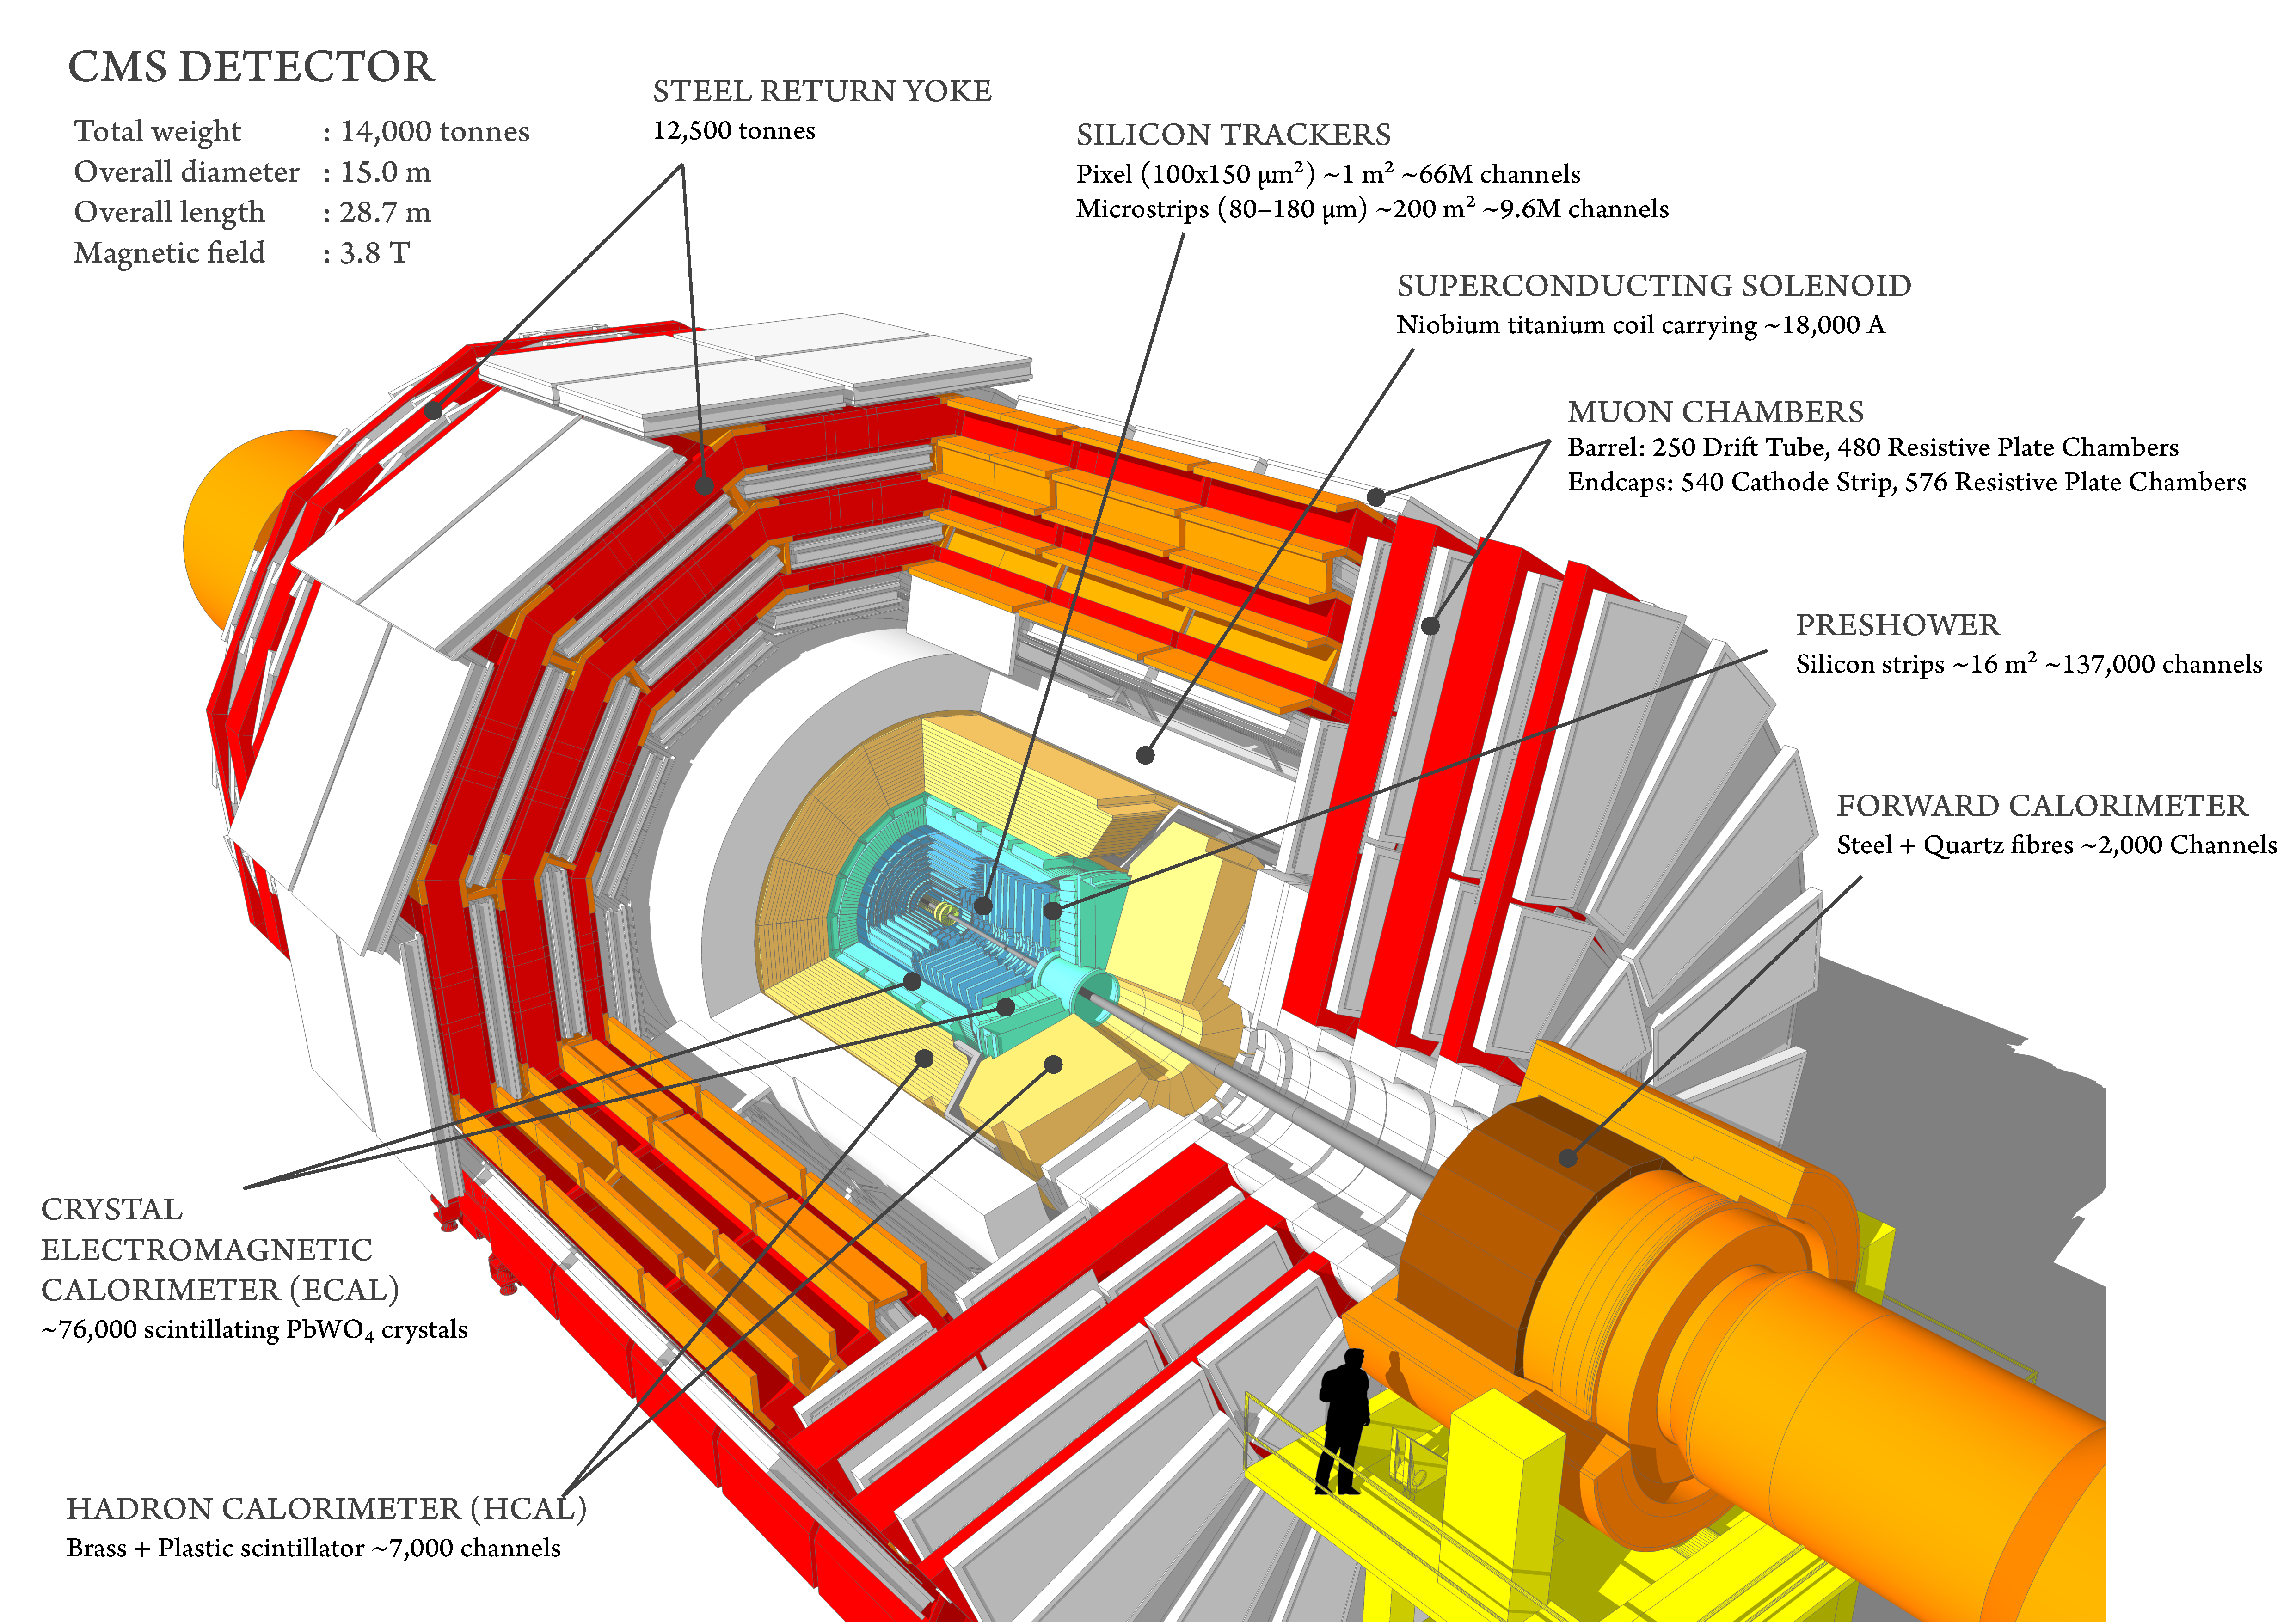
\includegraphics[width=0.9\textwidth]{figs/03_experiment/cms_160312_02.pdf}
	\caption[Cutaway diagram of CMS showcasing major detector components~\cite{Sakuma:2665537}.]
			{Cutaway diagram of CMS showcasing major detector components~\cite{Sakuma:2665537}.}
	\label{fig:CMS}
\end{figure}

\subsection{CMS Coordinate System} \label{sec:CMS_coord}
The origin of the CMS coordinate system is located at the center of the detector, at the nominal collision point of the proton beams. The $+\hat{x}$ axis points radially towards the center of the LHC, while the $+\hat{y}$ axis points vertically upward. This sets the $+\hat{z}$ direction along the beamline, counterclockwise along the LHC. Due to the cylindrical symmetry of CMS, coordinates in the $\hat{x}$-$\hat{y}$ plane are commonly replaced with the radius $r$ and the azimuthal angle $\phi$, which is measured from the positive $\hat{x}$-axis. The polar angle $\theta$ is measured from the $+\hat{z}$-axis, though in practice this variable is rarely used. It is more common to define the polar angle in terms of the pseudorapidity $\eta$, which is defined as
\begin{equation}
	\eta=\frac{1}{2}\ln\left(\frac{|\mathbf{p}|+p_{z}}{|\mathbf{p}|-p_{z}}\right)=-\ln{\tan\left(\frac{\theta}{2}\right)}
\end{equation}

The motivation for using $\eta$ instead of $\theta$ stems from a fundamental property of hadron colliders: the center of mass frame for particle production rarely coincides with the lab frame. Thus, when measuring the separation between particles, it is useful to define quantities that remain invariant under Lorentz transformations in the $\hat{z}$ direction. The rapidity $y$ (not to be confused with the Cartesian coordinate $\hat{y}$) is defined as
\begin{equation}
	y=\frac{1}{2}\ln\left(\frac{E+p_{z}}{E-p_{z}}\right)
\end{equation}
It is trivial to show that differences in $y$ remain invariant under Lorentz transformations. In the highly relativistic limit, which is valid for most particles produced at the LHC, rapidity approaches pseudorapidity as $E\approx|\mathbf{p}|$. One advantage of pseudorapidity is that $\eta$ can be calculated using only geometric quantities of the detector, whereas $y$ requires calculating both the energy and momenta of a particle, making pseudorapidity the natural choice for defining the polar angle. $\eta$ can range from $\left(-\infty, \infty\right)$, where $\eta=\pm\infty$ points directly along the $\pm\hat{z}$ axis. Higher values of $\left|\eta\right|$ are commonly referred to as "forward".

\subsection{Inner Tracker} \label{sec:CMS_tracker}
The CMS inner tracker is the first detector surrounding the primary interaction point (IP). Its purpose is to measure the tracks from charged particles as they curve in the strong magnetic field within CMS in order to calculate their momentum and reconstruct secondary vertices. As the closest detector to the primary IP, the tracker experiences the highest particle flux within CMS, and must have high enough granularity to distinguish the multitude of tracks. Additionally, particles passing through must lose minimal energy in order to maintain their trajectories into the outer detectors. The high flux also makes the detector susceptible to radiation damage, so the tracker must be robust in order to maintain efficiency over the long operational period of the LHC.

The inner tracker utilizes silicon tracking modules to detect the location of charged particles. When an external voltage is applied to a module, particles passing through will deposit energy and create electron-hole pairs, which drift to their respective electrodes and generate an electrical signal. The applied voltage is tuned such that only a small amount of energy is required to produce electron-hole pairs, which reduces the total amount of material required in order to minimize the energy loss of the charged particles. The inner layer of the tracker is composed of higher granularity pixel detectors, while the outer layer is composed of coarser silicon strips.

\subsubsection{Silicon Pixel Detector} \label{sec:CMS_pixel}
The pixel detector is comprised of 124 million silicon pixel sensors, each with an area of $100\times150\unit{\mu m^2}$ and a thickness of $300\unit{\mu m}$. The barrel (BPIX) consists of four cylindrical layers of pixel sensors spanning from $z=-54\unit{cm}$ to $z=54\unit{cm}$ at radii of $r=2.9$, $6.8$, $10.9$, and $16\unit{cm}$. The endcap (FPIX) consists of three layers located at $z=\pm29.1$, $\pm39.6$, and $\pm51.6\unit{cm}$, which when combined with the barrel nets a total sensitive area of $1.85\unit{m^2}$ with coverage up to $\abs{\eta}<2.5$. With regards to detector performance, the pixel detector provides spatial resolution of $9.5 \unit{\mu m}$ in the $r$-$\phi$ direction and $22.2 \unit{\mu m}$ in the $z$ direction, as well as a hit efficiency of $>99\%$ in each layer at nominal LHC luminosity, with the innermost BPIX layer dropping to $97.5\%$ at peak run 2 efficiency~\cite{CMSPixelP1}.

\begin{figure}[htbp]
	\centering
	\includegraphics[width=0.85\textwidth]{figs/03_experiment/20120828_01_pixel_phase1_largesharp.png}
	\caption
	[$r$-$z$ slice of the CMS pixel detector~\cite{CMSPixelP1}]
	{$r$-$z$ slice of the CMS pixel detector comparing original design (bottom, teal) with the Phase-I upgrade implemented in 2016/17, which added one layer to both the FPIX and BPIX (top, blue)~\cite{CMSPixelP1}.}
	\label{fig:pixel}
\end{figure}

\subsubsection{Silicon Strip Detector} \label{sec:CMS_strip}
The silicon strip detector surrounds the pixel detector, and is segmented into a tracker inner barrel (TIB), tracker outer barrel (TOB), tracker inner disks (TID), and tracker endcap (TEC). The TIB consists of four layers covering $\left|z\right|<65\unit{cm}$ and radius $25.5\unit{cm}<r<49.8\unit{cm}$. The endcaps of the TIB are covered by the TID, consisting of three disks covering $90<\left|z\right|<90\unit{cm}$. Surrounding the TIB is the TOB, with six layers spanning $\left|z\right|<188\unit{cm}$ and $60.8<\left|r\right|<108\unit{cm}$. Lastly, both the TOB and TID are closed by the TEC, which covers radii ranging from $22<r<113.5\unit{cm}$ and stretches from $124<\left|z\right|<280\unit{cm}$.

The strip detector modules function similarly to the pixel modules, but utilize much larger silicon strips due to the reduced particle flux compared to the pixel detector. Each strip detector is composed of $300\unit{\mu m}$ thick micro-strip sensors with pitch varying from $80-205\unit{\mu m}$ to form $7-12.5\unit{cm}$ long strip modules. Overall, the strip detector uses 15,148 modules covering an area of $200\unit{m^2}$ up to $\left|\eta\right|<2.5$.

\begin{figure}[htbp]
	\centering
	\includegraphics[width=0.85\textwidth]{figs/03_experiment/las.png}
	\caption
	[$r$-$z$ slice of the CMS silicon detector, detailing the four main components of the strip detector~\cite{Chatrchyan:1211825}]
	{$r$-$z$ slice of the CMS silicon detector, detailing the four main components (TIB, TOB, TID, and TEC) of the strip detector. Pixel detector is shown in its Run-I configuration~\cite{Chatrchyan:1211825}}
	\label{fig:strip}
\end{figure}

\subsection{Electromagnetic Calorimeter} \label{sec:CMS_ECAL}
The CMS Electromagnetic Calorimeter (ECAL) is designed to stop and capture the energy of photons and electrons. When a photon or election enters the ECAL, it interacts with the material in the detector through bremsstrahlung, $e^+e^-$ pair production, Compton scattering, or ionization, which in turn produce more photons or electseparaterons that continue these processes in a cascade that is referred to as an electromagnetic shower. The light produced from a shower is measured using photodetectors to determine the initial energy of the incident photon or electron, as the amount of light produced is proportional to the initial energy.

The material used for an electromagnetic calorimeter can be characterized by the radiation length ($X_0$) and moli\`ere radius ($R_M$). The radiation length is the average distance an electron will travel before its energy is reduced by a factor of $1/e$, and is roughly proportional to $A/Z^2$, where A is the atomic mass and Z is the atomic number. The moli\`ere radius directly proportional to the radiation length and measures the spread of an electromagnetic shower in the transverse direction. A low radiation length and moli\`ere radius ensure all of the energy is captured in the detector and is contained to a small area to precisely determine the position of an incident particle. It is for this reason that the CMS ECAL is composed of lead-tungstate (PbWO$_4$): a dense, high Z scintillator crystal with $X_0=7.39\unit{g/cm^2}$ (or $0.89\unit{cm}$ after dividing by the density of PbWO$_4$) and $R_M=2.2\unit{cm}$~\cite{Workman:2022ynf}.

The ECAL is constructed from 61200 + 15000 lead-tungstate crystals in the barrel + endcap region. Barrel crystals have a cross sectional area of $2.2\times2.2\unit{cm^2}$ to match the moli\`ere radius and a depth of 23$\unit{cm}$ (or $25.8 X_0$), and are arranged in rings along the $\phi$ direction, tilted to align with lines of constant $\eta$. The barrel has an inner radius of $129\unit{cm}$ and covers an eta region up to $\left|\eta\right|<1.479$. Endcap crystals have a slightly higher cross sectional area of $2.6\times2.6\unit{cm^2}$ and a slightly lower depth of 22$\unit{cm}$, and are arranged in an $x$-$y$ grid. The endcap provides the remaining coverage from $1.479<\left|\eta\right|<3.0$. Size and alignment of the crystals is designed to contain showers from incident photons/electrons within a $2\times2$ grid.

One common process in CMS is the production of $\pi^0$s, which decay to two photons. When the two photons deposit their energy into the ECAL, they can fake a signal from a single high energy photon. In the barrel, the two photons are generally separated by $\sim1\unit{cm}$, so the crystal granularity can be used to distinguish this background from real, high energy photons. However, $\pi^0$s in the forward region tend to be higher energy (commonly referred to as "more boosted"), resulting in separations on the order of millimeters. In order to identify these background events, a higher granularity detector known as a preshower is placed before the ECAL endcap. It consists of a layer of lead absorber to initiate the shower, followed by silicon strip sensors to measure the tracks within the shower. The lead has a thickness of $1.57\unit{cm}$ (or $2.8X_0$), thick enough to cause a shower while only causing energy loss of a few percent before the shower can reach the ECAL. The silicon strips are similar to those in the inner tracker, with a pitch of $1.9\unit{mm}$~\cite{TOURNEFIER2001355}.

\begin{figure}[htpb]
	\centering
	\includegraphics[width=0.85\textwidth]{figs/03_experiment/cms_ecal.pdf}
	\caption
	[Geometry of the CMS ECAL showing the barrel, endcap, and preshower, adapted from~\cite{Marzocchi2019}]
	{Geometry of the CMS ECAL showing the barrel, endcap, and preshower, adapted from~\cite{Marzocchi2019}}
	\label{fig:ecal}
\end{figure}


\subsection{Hadronic Calorimeter} \label{sec:CMS_HCAL}

\subsection{Muon Detectors} \label{sec:CMS_Muons}

\subsection{Trigger System} \label{sec:CMS_trig}

\subsubsection{Level-1 Trigger} \label{sec:CMS_L1T}

\subsubsection{High Level Trigger} \label{sec:CMS_HLT}

\subsection{Particle Flow} \label{sec:CMS_PF}
% !TEX = root../thesis.tex

\chapter{Real Time Muon Reconstruction at the Compact Muon Solenoid}
\label{chap:kbmtf}

\section{Introduction} \label{sec:kbmtf_intro}
Section~\ref{sec:CMS_L1T} provides an overview of the L1 trigger and its importance to the CMS trigger system. This section will detail the design and performance of a Kalman Filter algorithm used in the L1 trigger to identify muon tracks in the barrel region ($|\eta|<0.83$) of the CMS detector. This algorithm, known as the Kalman Barrel Muon Track Finder (KBMTF), was fully implemented for 2018 data taking and received improvements for continued use in Run-3.

The L1 barrel muon trigger receives inputs from the TwinMux system, which creates trigger primitives by combining information from the DT and RPC detectors to determine the position, trajectory, and timing of hits from incident muons at each station~\cite{Triossi_2017}. These hits, referred to as "stubs", are fed to the L1 muon trigger electrons where they are used to reconstruct muon tracks. The previous track finding algorithm, known as the Phase-I Barrel Muon Track Finder (BMTF), used a maximum of two stubs to reconstruct muon trajectories and was designed under the assumption that muons originate only from the beam line. As a part of upgrading the L1 Trigger, the KBMTF algorithm was developed to utilize stubs from all four muon stations as well as reconstruct displaced muon tracks resulting from decays of exotic long lived particles.

\section{The Kalman Filter Algorithm} \label{sec:kalman_filter}
A Kalman Filter is a tracking algorithm that performs a recursive, iterative chi-square-like fit. Qualitatively, it propagates a system from its current state to the next and combines the predicted value with measurements to "update" the state of the system. This updated system is then iteratively propagated and updated with new measured values. This section focuses on a discrete linear Kalman Filter, which is applicable when a system can be described with a vector of variables whose evolution can be modeled with a linear transformation plus random uncertainties~\cite{FRUHWIRTH1987444}.

Abstractly, the state of a system at a given step $n-1$ can be described by a vector labeled $x_{n-1}$ with covariance matrix $P_{n-1}$. Let the matrix $F_n$ represent the linear transformation that propagates $x_{n-1}$ to the next state $x_{n}$, and the matrix $Q_{n}$ be the covariance matrix due to additional uncertainty. The predicted state of the system at step $n$ can be given by
\begin{equation}
	\label{eq:prop}
	x_{n}=F_{n}x_{n-1} \quad \textrm{and} \quad P_{n}=F_nP_{n-1}F_n^T+Q_n
\end{equation}
where $F_nP_{n-1}F_n^T$ represents the propagation of the initial covariance matrix.

Now define a set of measurements taken at state $n$ as $z_n$ with covariance matrix $R_n$. The measured variables are not restricted to the same set of variables defining $x_n$ as long as there exist a "change of basis" matrix $H$ that relates the sets. It should be noted that mathematically $H$ is not a strict change of basis matrix, as the measured values can have smaller dimensionality than the propagated ones. The predicted state and covariance matrix of the system written in the same variables as the measured quantities are defined as
\begin{equation}
	\label{eq:changeOfBasis}
	\mu_n=Hx_n \quad \textrm{and} \quad \Sigma_n=HP_nH^{T}
\end{equation}

Updating the system relies on a matrix known as the Kalman Gain, which acts as a weight based on $\Sigma_n$ and $R_n$ and determines if the updated system should skew more towards the measured or predicted values. The Kalman gain is defined as
\begin{equation}
	\label{eq:gain}
	K\coloneqq \Sigma_n\left(\Sigma_n+R_n\right)^{-1}
\end{equation}
which is then used to calculate the updated system as follows
\begin{equation}
	\label{eq:update1}
	\mu_n'=\mu_n+K\left(z_n-\mu_n\right) \quad \textrm{and} \quad \Sigma_n'=\Sigma_n-K\Sigma_n
\end{equation}

The term $z_n-\mu_n$ is frequently referred to as the residual of the prediction and measured value. A Kalman gain equal to the identity $I$ would set the updated coordinates to the measured values, while a Kalman gain of $0$ would effectively ignore the measured values. Finally, we substitute $x_n$ and $P_n$ into equation~\ref{eq:update1} using equation~\ref{eq:changeOfBasis} and simplify to give
\begin{equation}
	x_n'=x_n+K'(z_n-Hx_n) \quad \mathrm{and} \quad P_n'= P_n-K'HP_n
\end{equation}
where the Kalman Gain $K$ has been redefined to
\begin{equation} \label{eq:gain2}
	K'=P_nH^T(HP_nH^T+R_n)^{-1}
\end{equation}
The system $x_n'$ and $P_n'$ can now be propagated to step $n+1$ where the Kalman Algorithm can be iterated.

\section{The Kalman Barrel Muon Track Finder} \label{sec:kbmtf}
A rough outline KBMTF algorithm for track finding is as follows:
\begin{enumerate}
	\item A track seed is chosen from a stub in the muon station, from which a preliminary track is built. This seed cannot be chosen from the innermost muon station.
	\item The track is propagated inward to the next station and matched to the closest stub. If there is a matching stub, update the track with the stub information. Repeat until the track is at the innermost station. \label{kbmtf_step2}
	\item The track is propagated from the innermost station to the beamline. The track properties at this point are stored as the "vertex unconstrained" measurement. These properties include the $p_T$, $\phi$, $\eta$, and $d_{xy}$, which is defined as the closest distance from the propagated track to the beamline. \label{kbmtf_step3}
	\item The vertex propagated track is updated with the constraint that the track originated from the beamline, and the track properties are stored as the "vertex constrained" measurement. \label{kbmtf_step4}
\end{enumerate}

Muon track finding begins at the outer stations in order to get both the vertex unconstrained measurement and the vertex constrained measurement with only one iteration of the KBMTF algorithm. Starting from the inner station and propagating outward would require an additional propagation back inward in order to get the vertex constrained measurement, which would cause the algorithmic latency to exceed timing restrictions. The outer stations are also the lowest occupancy, meaning stubs are less likely to be from background. Tracks are then overlap cleaned, which ensures that stubs are not shared among multiple tracks, and cut and selected based on various goodness of fit criteria. A diagram showing the KBMTF propagation and update procedure can be shown in figure~\ref{fig:kbmtf}.

\begin{figure} [htb!]
	\centering
	\includegraphics[width=0.85\linewidth]{figs/04_muons/kbmtf_diagram.png}
	\caption[The iterative process of propagation and updating a muon track through the KBMTF algorithm. The track properties at the innermost station are stored in order to trigger on muons not originating from the beamline~\cite{CERN-LHCC-2020-004}]
	{The iterative process of propagation and updating a muon track through the KBMTF algorithm. The track properties at the innermost station are stored in order to trigger on muons not originating from the beamline~\cite{CERN-LHCC-2020-004}.}
	\label{fig:kbmtf}
\end{figure}

\subsection{Muon Trajectory Propagation} \label{sec:muons_prop}
In order to implement a Kalman Filter, the propagation of muon tracks between stations must be expressed as a linear function of the track variables. From equation~\ref{eq:pt03br}, a charged particle will travel in a circular orbit in the $\hat{r}-\hat{\phi}$ plane. The high center of mass energy of the LHC results in highly energetic particles, whose trajectories have radii substantially larger than the size of the CMS detector. The large radius of curvature allows us to approximate these trajectories as parabolas. Assume a Cartesian coordinate system with the origin placed along a particle's trajectory that has radius R. This trajectory can then be approximated as
\begin{equation}
	\label{eq:parabola1}
	y(x)=\frac{x^2}{2R}+bx
\end{equation}
where $b$ is a coefficient depending on the orientation of the coordinate system. If the initial trajectory is defined as $\phi_{b,0}$, taking the derivative and evaluating at the origin yields
\begin{equation}
	\label{eq:phib}
	y'(0)=\tan(\phi_{b,0})=b
\end{equation}	
The curvature $k=q/p_{T}$, where the muon charge $q=\pm1$, is the preferred variable to work with when propagating the trajectory of a muon, as the propagation is linear in $k$. Substituting values from equations~\ref{eq:pt03br} and~\ref{eq:phib} into equation~\ref{eq:parabola1} yields
\begin{equation}
	\label{eq:parabola2}
	y(x)=akx^2+\tan(\phi_{b,0})x
\end{equation}
where $a=\frac{0.3B}{2}$. Muon hits, or "stubs", provide information on the position $\phi$ and bending angle $\phi_b$. Let the radius of two sequential muon stations be $r_1$ and $r_2$, with the outer radius given by $r_2$ and $\Delta r=r_2-r_1$. Assuming a muon has curvature $k$ at the outer station and ignoring energy loss, equation~\ref{eq:parabola2} can be used to propagate stubs from the outer station towards the inner station.
\begin{equation}
	y(-\Delta r) = \left(a\Delta r^2\right)k-\Delta r\tan(\phi_{b,0})
\end{equation}
\begin{equation}
	y'(-\Delta r)=-\left(2a\Delta r\right)k+\tan(\phi_{b,0})
\end{equation}
Converting these to the quantities to angles measured by the detector yields
\begin{equation}
	\label{eq:prop_phi}
	\tan(\Delta\phi)=\frac{y(-\Delta r)}{r_1}
\end{equation}
\begin{equation}
	\label{eq:prop_phib}
	\phi_b=\Delta\phi+\mathrm{tan}^{-1}\left[y'(-\Delta r)\right]
\end{equation}
The $\Delta\phi$ term is added to equation~\ref{eq:prop_phib} because the bending angle at each station is measured relative to an axis system oriented towards the center of the detector. Due to the large radius of curvature of the muon trajectories, the small angle approximation $\tan(x)\sim \tan^{-1}(x)\sim x$ can be applied, giving the equations
\begin{equation}
	\label{eq:prop_phi_approx}
	\Delta\phi=\frac{a\Delta r^2}{r_1}k-\frac{\Delta r}{r_1}\phi_{b,0}
\end{equation}
\begin{equation}
	\label{eq:prop_phib_approx}
	\phi_b=a\Delta r\left(\frac{\Delta r}{r_1}-2\right)k+\left(\frac{r_2}{r_1}\right)\phi_{b,0}
\end{equation}
A diagram showing this propagation can be seen in figure~\ref{fig:mu_trajectory}.

\begin{figure}[h!]
	\centering
	%Final image: origin at outer stub, oriented with x axis pointing towards vertex
	\begin{tikzpicture}
		% axis system
		\draw[thick,->] (-11, 0) -- (1, 0) node[anchor=west] {x};
		\draw[thick,->] (0, 0) -- (0, 4) node[anchor=south] {y};
		\coordinate[label = above left:$\mathrm{Vertex}$] (vertex) at (-9.5, 0);
		\coordinate[label = above right:$\mathrm{Origin}$] (origin) at (0, 0);
		\coordinate[] (r1) at (-5, 0);
		\node at (vertex)[circle,fill,inner sep=2pt]{};
		\node at (origin)[circle,fill,inner sep=2pt]{};
		\draw[<->] (-9.5, -.5) -- (-5, -.5);
		\draw[<->] (-9.5, -1.1) -- (0, -1.1);
		\coordinate[label = below:$r_1$] (r1) at (-7.25,-.5);
		\coordinate[label = below:$r_2$] (r2) at (-5,-1.1);
		\draw[dashed] (-5, 0) -- (-5, 4);
		
		% muon trajectory
		\def \X{2.6047227}; %circle x0
		\def \Y{14.772116}; %circle y0
		
		\def \sy{1.8427620};%stub at (-5, y)
		\draw [{Latex[length=3mm]}-, domain=270:230] plot ({\X+15*cos(\x)}, {\Y+15*sin(\x)});
		\draw ({\X+15*cos(230)}, {\Y+15*sin(230)}) node[font=\bfseries, anchor=east] {$\mu$};
		\draw (-2.25,.25) node[anchor=west] {$\phi_{b,0}$};
		\coordinate[] (stub1) at (-5, \sy);
		\draw [dashed, domain=0:6] plot ({-9.5+\x}, {0.40950267*\x});
		\draw [dashed] (-5, \sy) -- (-4, \sy);
		\draw (-8.5, .25) node[anchor=west] {$\Delta\phi$};
		\draw (-4, \sy) node[anchor=west, scale=1.0] {$\phi_b$};
		\draw (-4.5, \sy+.1) node[anchor=west, scale=0.7] {$\Delta\phi$};
	\end{tikzpicture}
	\caption{Diagram showing a muon trajectory between two stations with the origin set at the outer station. The x-axis is oriented using the detector vertex and the outer station.}
	\label{fig:mu_trajectory}
\end{figure}

Equations~\ref{eq:prop_phi}-\ref{eq:prop_phib} show that the track propagation fits the criteria for a discrete linear Kalman Filter discussed in section~\ref{sec:kalman_filter}. The matrices for propagation can now be constructed as follows. The transfer matrix $F_n$ from equation~\ref{eq:prop} can be expressed as
\begin{equation}
	\label{eq:kmtfProp}
	x_{n}=\left(\begin{matrix}
		k\\
		\phi\\
		\phi_b
	\end{matrix}\right)_{n} = 
\left(\begin{matrix}
	1 & 0 & 0\\
	\alpha_n & 1 & -\frac{\Delta r}{r_n}\\
	\beta_n & 0 & \frac{r_{n-1}}{r_n}
\end{matrix}\right)
\left(\begin{matrix}
	k\\
	\phi\\
	\phi_b
\end{matrix}\right)_{n-1}=F_nx_{n-1}
\end{equation}
where the coefficients
\begin{equation}
	\label{eq:kmtf_coeff}
	\alpha_n=a\frac{\Delta r^2}{r_n} \quad \mathrm{and} \quad \beta_n=a\Delta r\left(\frac{\Delta r}{r_n}-2\right)
\end{equation}
with $r_{n-1}$ being the radius of the previous (outer) muon station and $r_n$ the radius of the sequential (inner) muon station.

While the radii of the muon stations are determined by detector geometry, the constants $\alpha_n$ and $\beta_n$ are measured using single muon monte-carlo samples where stubs are matched to the incident muons using generator level information. To determine $\alpha_n$, stubs in stations $n$ and $n-1$ are first associated if they resulted from the same incident muon. For matching stubs, the quantity $\Delta\phi+\frac{\Delta r}{r_1}\phi_{b,0}$ is plotted versus the muon $k$ in a 2-dimensional histogram. Slices along the y-axis are fit using a Gaussian distribution, and the mean value for each slice is used to calculate a linear fit as a function of $k$. $\beta_n$ is calculated similarly by plotting $\phi_b-\left(r_{n-1}/r_n\right)\phi_{b,0}$ vs $k$. This process can be seen in figure~\ref{fig:phi_prop}.

\begin{figure}[htb!]
	\centering
	\captionsetup{justification=centering}
	\begin{subfigure}[b]{0.45\textwidth}
		\centering
		\includegraphics[width=\textwidth]{figs/04_muons/phiprop_2d.pdf}
		\caption{2-dimension histogram of $\Delta\phi+\frac{\Delta r}{r_1}\phi_{b,0}$ vs $k$.}
		\label{fig:2dprop}
	\end{subfigure}\hspace{0.05\textwidth}
	\begin{subfigure}[b]{0.45\textwidth}
		\centering
		\includegraphics[width=\textwidth]{figs/04_muons/phiprop_mean.pdf}
		\caption{Mean of vertical slices fits used to calculate $\alpha$.}
		\label{fig:2dprop_mean}
	\end{subfigure}
	\caption[Calculation of phi propagation coefficients. Units are converted to their digitized form used in firmware calculations.]
	{Calculation of phi propagation coefficients. Units are converted to their digitized form used in firmware calculations.}
	\label{fig:phi_prop}
\end{figure}

\subsection{Covariant Matrices and the Kalman Gain} \label{sec:kbmtf_cov}
There are two sources of uncertainty that affect the covariance matrices. The first is multiple coulomb scattering, which occurs when muons scatter elastically with material in the detector. This can be thought of as a small deflection in momentum that alters the trajectory the muon. Lower momentum muons will be deflected at greater angles, so this uncertainty is proportional to $k$. Additionally, the probability for multiple scattering is proportional to the amount of material traversed by the muon, so this uncertainty must be calculated for each step in propagation. This is an uncertainty resulting from the propagation, and therefore plays the role of $Q_n$ from equation~\ref{eq:prop}. The second source is from the intrinsic detector resolution, which is a fixed value for each detector. However, the angular resolution is dependent on the radial distance from the center of the detector, so these must be calculated for each station as well. Since this is an uncertainty on the measurements, the resolution plays the role of $R_n$ in equation~\ref{eq:gain}. The total uncertainty resulting from both of these factors is given by
\begin{equation}
	\label{eq:prop_uncertainty}
	\sigma(k)=\sqrt{\sigma_{ms}^2k^2+\sigma_{res}^2}
\end{equation}

The coefficients can be calculated by using the Gaussian slice fits described when deriving $\alpha$ and $\beta$. For each propagation, the sigma of the Gaussian fits is plotted versus $k$ and fit to the form in equation~\ref{eq:prop_uncertainty}. This fitting process for $\phi$ propagation coefficients is shown in figure~\ref{fig:phi_uncertainty}, and is functionally the same for $\phi_b$.

\begin{figure}[htb!]
	\centering
	\includegraphics[width=0.45\linewidth]{figs/04_muons/phiprop_sigma.pdf}
	\label{fig:2dprop_sigma}
	\caption[$\sigma$ of vertical slice fits of the 2-dimensional histogram in figure~\ref{fig:2dprop} used to calculate uncertainty coefficients.]
	{$\sigma$ of vertical slice fits of the 2-dimensional histogram in figure~\ref{fig:2dprop} used to calculate uncertainty coefficients.}
	\label{fig:phi_uncertainty}
\end{figure}

Each stub has a measured value representing the "quality" of the hits, with higher values representing a more precise reconstruction of the bending angle. For this reason, the $\phi_b$ position resolutions are calculated separately for high and low quality stubs, as the uncertainty can differ by over a factor of 10 between the two. 

Since the muon detectors only measure $\phi$ and $\phi_b$, the matrix $H$ described in equation~\ref{eq:changeOfBasis} must be a 2$\times$3 matrix that takes the form
\begin{equation}
	H=\left(\begin{matrix}
		0 & 1 & 0\\
		0 & 0 & 1\end{matrix}\right)
\end{equation}

From this, the Kalman Gain $K'$ defined in equation~\ref{eq:gain2} must be a 3x2 matrix with indices $K_{ij}$, and the update step can be explicitly written as
\begin{equation} \label{eq:kmtfUpdate}
	\begin{split}
		k_n^\mathrm{upd}=k_{n-1}+K_{00}\Delta\phi+K_{01}\Delta\phi_b \\
		\phi_n^\mathrm{upd}=\phi_n^\mathrm{prop}+K_{10}\Delta\phi+K_{11}\Delta\phi_b \\
		\phi_{b,n}^\mathrm{upd}=\phi_{b,n}^\mathrm{prop}+K_{20}\Delta\phi+K_{21}\Delta\phi_b
	\end{split}
\end{equation}
where $\Delta\phi$ and $\Delta\phi_b$ are the residuals for $\phi$ and $\phi_b$.

\subsection{Firmware Implementation of the KBMTF} \label{sec:fw}

Two minor approximations are made in order to reduce algorithmic latency and memory usage for firmware implementation. The position resolution of $\phi$ is substantially smaller than the multiple scattering resolution, so the track $\phi$ is set automatically to the measured stub $\phi$. This is equivalent to fixing $K_{10}=1$ and $K_{11}=0$ in equation~\ref{eq:kmtfUpdate}. Secondly, due to the high uncertainty associated with both the measured and propagated $\phi_b$, tracks using three or more stubs set $K_{i1}$ equal to zero and only update using the residual from $\phi$.

Although the Kalman Gain can be exactly calculated exactly given the covariance matrices using equation~\ref{eq:gain}, matrix inversion is a resource and latency expensive process for the hardware based trigger. Implementing division into hardware is significantly more resource intensive than multiplication, so the calculation of the determinant for matrix inversions would cause the algorithm to exceed the latency requirements for real time track finding. Instead, the values of $K_{ij}$ are stored in look-up tables (LUTS) as a function of curvature and the combination of stations that were used to update the track, referred to as the track pattern. For tracks with only two stubs, the LUT contains the exact values of the gain that would have been calculated using equation~\ref{eq:gain2}. For tracks with more than two stubs, this is an approximation that loses some information from updates at previous stations but produces nearly identical performance.

As outlined in section~\ref{sec:kbmtf_cov}, the $\phi_b$ resolution coefficients are different for high and low quality stubs, thus the values for $K_{ij}$ would have to be provided for every possible combination of high and low quality stubs for each track pattern. This would exponentially increase the number of gains stored on LUTs beyond the memory capacity of the hardware. However, from previous approximations, residuals for $\phi_b$ are not used for tracks containing three or more stubs, which fixes $K_{01}$ and $K_{21}$ at 0 for these track patterns. Only gains for track patterns containing two stubs must account for the quality of the stubs. With four stations, this yields six track patterns with four combinations of stub quality that must be stored in LUTs, which is within the capacity of the current hardware.

The firmware is written using Vivado High Level Synthesis (HLS) which compiles firmware written in C to HDL, optimizing it for a given FPGA and clock frequency~\cite{Bachtis:2648953}. When synthesized in a Virtex 7 690T FPGA with a clock frequency of 160\unit{MHz}, the KBMTF algorithm can process a single event in 9 bunch crossings, and is pipelined to allow for continuous processing of events. Table~\ref{tab:kmtfFW} shows the resource utilization of the KBMTF compared to the previous BMTF algorithm, which was implemented using an identical FPGA and clock frequency.

\begin{table} [h!]
	\centering
	\begin{tabular}{|l|r r r r|}
	\hline
	Algorithm & LUT & FF & BRAM & DSP \\
	\hline
	Phase I BMTF & 43\% & 23\% & 35\% & 0\%\\
	KBMTF & 16\% & 11\% & 15\% & 25\% \\
	\hline 
	\end{tabular}
	\caption[Comparison of FPGA resource utilization~\cite{CERN-LHCC-2020-004}. The KBMTF utilizes DSP cores for arithmetic operations to propagate and update tracks and LUTs for the propagation coefficients and approximate Kalman Gain, while the BMTF uses LUTs to assign momentum.]
	{Comparison of FPGA resource utilization~\cite{CERN-LHCC-2020-004}. The KBMTF utilizes DSP cores for arithmetic operations to propagate and update tracks and LUTs for the propagation coefficients and approximate Kalman Gain, while the BMTF uses LUTs to assign momentum.}
	\label{tab:kmtfFW}
\end{table}

\section{Performance of the Kalman Barrel Muon Track Finder} \label{sec:kmtf_performance}
The performance of an trigger algorithm is primarily determined by the rate and efficiency. The efficiency is the fraction of signal events that successfully have a track reconstructed by the algorithm, while the rate is the frequency that the algorithm will trigger. A high efficiency is desirable to ensure any interesting events are stored for future analysis, while a low rate is crucial to reject background events and provide a reasonable bandwidth to store events.

\subsection{Trigger Efficiencies and Rate} \label{sec:kmtf_eff}
The previous L1 barrel muon trigger (BMTF) functioned by using pairs of stubs to form tracks, then using a LUT to assign track parameters based on the $\phi$ and $\phi_b$ of the stubs. This LUT takes only the $\phi$ and $\phi_b$ of the two stubs and was calculated with the assumption that the muon originated from the beamspot. In the case of displaced muons, which arise from secondary decays of long lived, beyond standard model particles, the assumption is no longer valid and results in large inefficiencies as the muon becomes more displaced from the beamspot.

The general efficiency of a trigger is defined as the fraction of signal muons that have a matching reconstructed track, and can be expressed abstractly as

\begin{equation}\label{eq:eff}
	\epsilon=\frac{N_\mathrm{signal}(\mathrm{Passing\ trigger})}{N_\mathrm{signal}}	
\end{equation}

For muon triggers, the denominator of signal muons consist of events that have known information about the muons. This can be from generator information in simulated monte-carlo samples, tracker information using cosmic muon data, or probe muons using the tag-and-probe method on data. These signal muons are cut using the known muon information to produce a reasonable sample for track reconstruction. The numerator consists of signal muons with a matching reconstructed track that may have addition cuts on the reconstructed track properties.

Figure~\ref{fig:effVsDxy_kmtf} shows the efficiency versus muon $d_{xy}$ for three track finding algorithms. The denominator consists of cosmic ray muons passing through the barrel muon detectors with a $p_T>20\unit{GeV}$. The numerator requires a matching L1 track with reconstructed $p_T>10\unit{GeV}$. The lower threshold for the L1 track is set to prevent the momentum resolution of the reconstruction algorithms from affecting the efficiency. The first algorithm is the BMTF, which shows inefficiencies due to the $p_T$ LUTs assuming the muon originated at the beamspot. The second is the prompt KBMTF, which uses the vertex constrained measurement. This also shows inefficiencies due to the vertex constraint, but is better than the BMTF as the vertex constraint isn't applied until the last step of track reconstruction. Lastly, the displaced KBMTF uses the vertex unconstrained measurement and shows substantial improvements compared to both prompt algorithms.

\begin{figure}[htbp!]
	\centering
	\includegraphics[width=0.5\linewidth]{figs/04_muons/effVsDxy_kmtf.png}
	\caption[Comparison of efficiency vs cosmic track $d_{xy}$ using cosmic data from the 2018 data taking run. The prompt KBMTF takes the reconstructed $p_{T}$ using the vertex constrained measurement, while the displaced KBMTF uses the veretx unconstrained measurement. The displaced KBMTF shows substantial improvements to the previous BMTF~\cite{Hayrapetyan:2870088}]
	{Comparison of efficiency vs cosmic track $d_{xy}$ using cosmic data from the 2018 data taking run. The prompt KBMTF takes the reconstructed $p_{T}$ using the vertex constrained measurement, while the displaced KBMTF uses the veretx unconstrained measurement. The displaced KBMTF shows substantial improvements to the previous BMTF~\cite{Hayrapetyan:2870088}.}
	\label{fig:effVsDxy_kmtf}
\end{figure}

A reconstructed track must have a $p_T$ above a given threshold to trigger on an event. Thresholds are set to optimize the analysis potential of the data while also minimizing the additional bandwidth to store events. The rate, which is the frequency at which a trigger decides to store an event, can be calculated as a function of threshold using zero bias data, which is collected by storing random events regardless of trigger acceptance. This creates a representative data set of all $pp$ collisions, hence the name "zero bias". The rate can be calculated from the zero bias data as follows
\begin{equation}
	\mathrm{R} = f_\mathrm{rev}\times \left<N_\mathrm{bunches}\right>\times\frac{N_\mathrm{events}(\mathrm{L1}\ \mathrm{Track}\ p_{T}>\mathrm{Threshold})}{N_\mathrm{events}}
\end{equation}
Where $f_\mathrm{rev}$ is the LHC revolution frequency of 11.245\unit{kHz} and $\left<N_\mathrm{bunches}\right>$ is the average number of proton bunches that will collide in one revolution. For 2017 data taking these yield a scale factor of 20984$\unit{kHz}$. Figure~\ref{fig:kmtf_rate} shows the rate versus threshold for the BMTF, vertex constrained KBMTF, and vertex unconstrained KBMTF.

\begin{figure}[htbp!]
	\centering
	\includegraphics[width=0.5\linewidth]{figs/04_muons/rate_kmtf.pdf}
	\caption[Rate comparison calculated using 2017 zero bias data of the Phase I BMTF, vertex constrained (prompt) KBMTF, vertex unconstrained (displaced) KBMTF, and displaced KBMTF for displaced tracks.]{Rate comparison calculated using 2017 zero bias data of the Phase I BMTF, vertex constrained (prompt) KBMTF, vertex unconstrained (displaced) KBMTF, and displaced KBMTF for displaced tracks.}
	\label{fig:kmtf_rate}
\end{figure}

\subsection{Firmware and Emulator Agreement} \label{sec:kmtf_fwVsEmu}
The performance of the KBMTF is tested using a dedicated C++ software emulator which is integrated into the CMS analysis framework. This emulator follows similar logic to the HLS code, but is not a one-to-one replica. Several modifications are made to the HLS code in order to make it compatible with the synthesis into HDL and pipelining. As such, a test bench is used to ensure that the output of the firmware and emulator are identical. The emulator runs the algorithm over several events and outputs a text file containing information on the input stubs and the reconstructed tracks. This text file is used as input for the test bench, which runs the stub information through the HLS code and compares the properties of the reconstructed tracks to those found in the emulator.

Disagreements between the emulator and firmware are used for a variety of debugging purposes. They frequently point to logic errors in the simplification of the algorithm for HLS synthesis, or in other cases show flaws in the emulator. During Run 2, the disagreements were almost entirely due to differences resulting from fixed point calculations in the firmware compared to floating point calculations in the emulator. These differences have been drastically reduced due to the addition of C++ classes that mimic fixed point calculations in the emulator, which now has a $>$99.9\% agreement to the firmware. Figure~\ref{fig:kmtf_rate} shows a comparison of the outputs of the firmware and emulator using events from a 2017 Z tag-and-probe sample.

\begin{figure}[htb!]
	\centering
	\includegraphics[width=0.55\linewidth]{figs/04_muons/emuVsFw_pt.pdf}
	\caption[Comparison of the track $p_T$ between the firmware and emulator using data from a 2017 Z tag-and-probe sample. hwPt represents the integer value of p$_T$ used in hardware. The emulator and firmware output show 100\% agreement across 500000 events.]{Comparison of the track $p_T$ between the firmware and emulator using data from a 2017 Z tag-and-probe sample. hwPt represents the integer value of p$_T$ used in hardware. The emulator and firmware output show 100\% agreement across 500000 events.}
	\label{fig:kmtf_fwVsEmu}
\end{figure}

\section{The Phase-2 KBMTF} \label{sec:HL_KBMTF}
The modifications to the KBMTF algorithm for the HL-LHC result from increased precision from the input trigger primitives and modifications to the trigger architecture. These changes mainly affect the firmware implementation and do not require conceptual changes to the logic used to propagate and update tracks. The propagation coefficients and Kalman Gain must be recalculated as the number of bits allocated to $k$, $\phi$, and $\phi_b$ change. Additionally, the firmware will receive primitives from the entire barrel muon system simultaneously as opposed to processing each sector in $\phi$ independently. The firmware will be time-multiplexed with a factor of 18, meaning data from each event will be sent to one of 18 processors running the KBMTF algorithm in parallel. Additionally, the FPGA will be changed to a ZYNQ Ultrascale+ and synthesized at a clock frequency of 200\unit{MHz}. Simulations show a resource utilization of 17\% LUT, 3\% FF, 11\% DSP, and 7\% BRAM~\cite{CERN-LHCC-2020-004}.

The KBMTF algorithm performance is robust to the high pileup conditions of the HL-LHC. The efficiencies remain the same as Phase-1, and the rate scales approximately linearly with pileup as expected. Figure~\ref{fig:rate_eff_HLLHC} shows the efficiency versus generated muon $p_T$, single muon rates versus threshold, and single muon rates versus pileup for the Phase-2 KBMTF and two proposed track finding algorithms. As discussed in section~\ref{sec:CMS_L1T}, the HL-LHC track trigger introduces new track primitives that will be used in novel muon triggers. These new algorithms have higher efficiency and precision for prompt muons due to the momentum resolution of the tracker, but will be unable to trigger on displaced muons as the track primitives do not include displaced tracks. 

\begin{figure} [htb!]
	\centering
	\captionsetup[subfigure]{justification=centering}
	\begin{subfigure}[h]{0.45\linewidth}
		\centering
		\includegraphics[width=\linewidth]{figs/04_muons/effVsPt_20_TPS.pdf}
		\caption{Efficiency vs gen $\mu$ $p_T$.}
		\label{}
	\end{subfigure} \hspace{0.05\linewidth}
	\begin{subfigure}[h]{0.45\linewidth}
		\centering
		\includegraphics[width=\linewidth]{figs/04_muons/rateVsPt_TPS.pdf}
		\caption{Single muon rates versus threshold.}
		\label{}
	\end{subfigure}
	\begin{subfigure}[h]{0.45\linewidth}
		\centering
		\includegraphics[width=\linewidth]{figs/04_muons/rateVsPU_TPS.pdf}
		\caption{Single muon rates vs pileup for a 20\unit{GeV} threshold~\cite{CERN-LHCC-2020-004}}
		\label{}
	\end{subfigure}
	\caption[Performance of the L1 Barrel Muon algorithms using simulated samples with HL-LHC run conditions. The Track + KBMTF algorithm matches tracks to loose KBMTF muons, while the L1 Track + Muon Stubs algorithm matches tracks to muon stubs.]{Performance of the L1 Barrel Muon algorithms using simulated samples with HL-LHC run conditions. The Track + KBMTF algorithm matches tracks to loose KBMTF muons, while the L1 Track + Muon Stubs algorithm matches tracks to muon stubs.}
	\label{fig:rate_eff_HLLHC}
\end{figure}
% !TEX = root../thesis.tex

\chapter{Search for a Long Lived Scalar Boson}
\section{Introduction} \label{sec:ana_intro}
This chapter describes the search for beyond the standard model (BSM) particles using data taken by the CMS detector from 2016-2018. The following sections outline the choice of datasets and simulated samples, event selection criteria, methods of background estimation and statistical analysis for signal extraction, and results.

\section{Data and Simulated Samples} \label{sec:ana_samples}

\subsection{Data Samples} \label{sec:ana_data}
As discussed in chapter~\ref{chap:exp}, interesting events that pass at least 1 HLT path are stored for future analysis. These events are collected and sorted into datasets based on the number, flavor, and type of physics objects used in the HLT path. It can be noted that these datasets are not disjoint; one event can be sorted into multiple datasets if it satisfies more than a single HLT path. This data is maintained and updated by the Physics Data and Monte Carlo Validation (PdmV) group, which also provides recommendations on optimal usage for physics analysis~\cite{pdmv}. This search utilizes the PdmV recommended datasets for Run-2 analyses, referred to as Ultra-Legacy (UL), which has been reprocessed using the most current calibration for detector responses and alignment. Although the characteristic signature of this analysis is two displaced photons, the HLT double photon triggers present in Run-2 are unsuitable for the phase space of signal photons. Therefore we utilize the leptonic decay of the associated \VZ which provides a robust trigger. Since we are interested in \VZ decays to either electrons or muons, we use the datasets labeled as SingleMuon or SingleElectron (renamed to EGamma in 2018).

The reprocessed datasets must be cross referenced with the "Golden JSON": a certificate created by the Data Quality Monitoring (DQM) group within CMS by monitoring each sub-detector system in order to veto collisions that occur during sub-optimal conditions. The total integrated luminosity recorded by CMS during Run-2 was $164\unit{fb^{-1}}$; however, only $138\unit{fb^{-1}}$ of that was certified for analysis. The total integrated luminosity and uncertainty per year for collisions recommended by DQM can be seen in table~\ref{tab:intLumi}.

\begin{table}[h]
	\centering
	\caption[Table of integrated luminosity per year~\cite{cmslumi2016,cmslumi2017,cmslumi2018}.]{Table of integrated luminosity per year~\cite{cmslumi2016,cmslumi2017,cmslumi2018}.}
	\label{tab:intLumi}
		\begin{tabular}{l|l|l|l|l}\hline
			Year & 2016 & 2017 & 2018 & 2016-2018\\
			\hline
			\hline
			Luminosity $[\text{fb}^{-1}]$ & 36.31 & 41.48 & 59.83 & 137.62\\
			\hline	
			Uncertainty $[\%]$ & 1.2 & 2.3 & 2.5 & 1.6\\
			\hline
		\end{tabular}
\end{table}

\subsection{Simulated Samples} \label{sec:ana_mc}
Simulated samples use Monte Carlo methods to generate events in several steps, starting from the matrix elements that determine cross sections and hadronization processes and ending with the processing of digitized signals from each subdetector in CMS. These samples are generally created to model specific physics processes such as Drell-Yan, QCD, $t\bar{t}$, etc. Simulated events are not created one-to-one to match data events; instead they are used to create weighted events that are normalized to match the luminosity of the data. For this analysis we use both simulated background events as well as simulated signal samples.

\subsubsection{Monte Carlo Background} \label{sec:ana_mcbkg}
Although this analysis employs a data driven method of background estimation, simulated samples are used to inform on properties of background events and tune cuts to discriminate between signal and background. For this analysis, we use simulated Drell-Yan (DY) events with 0, 1 and 2 additional jets, simulated using matrix elements calculated at next-to leading order (NLO). Studies were done with inclusive (any number of additional jets) samples but found to have worse agreement and statistical power compared to the jet categorized samples.

\section{Event Selection} \label{sec:ana_eventsel}

\begin{appendices}
	\input{chapters/A1_QFT.tex}
\end{appendices}
\bibliography{bib/articles,bib/misc,bib/books,bib/reports}
\bibliographystyle{unsrturl}

\end{document}